\documentclass[11pt]{beamer}
\usepackage{pifont}
\usepackage[english]{babel}
\usepackage[backend=biber,style=numeric-comp,sorting=none]{biblatex}
\usepackage{graphicx}
\usepackage{subcaption}
\usepackage{csquotes}

\addbibresource{biblio.bib}

\definecolor{kyushu}{RGB}{133, 2, 62}
\setbeamercovered{transparent}
\setbeamertemplate{itemize items}{\ding{108}}
\setbeamercolor{itemize item}{fg=kyushu}
\setbeamertemplate{itemize subitem}{--}
\setbeamercolor{itemize subitem}{fg=black}
\setbeamerfont{frametitle}{series=\bfseries}
\setbeamercolor{frametitle}{bg=kyushu, fg=white}
\setbeamercolor{title}{
	bg=kyushu, fg=white
	%\hspace*{-\Gm@lmargin}
	%\hspace*{-\Gm@lmargin}
	%\begin{beamercolorbox}[wd=\paperwidth,ht=4.5ex,dp=2ex,leftskip=0.5cm]{frametitle}
			%\usebeamerfont{frametitle}
	%\begin{beamercolorbox}[wd=\paperwidth,ht=4.5ex,dp=2ex,leftskip=0.5cm]{frametitle}
			%\usebeamerfont{frametitle}
}
\addtobeamertemplate{frametitle}{}{%
	\begin{picture}(0, 0)
		\put(\textwidth, 25){\makebox(0, 0)[r]{\small\insertframenumber}}
	\end{picture}
}

\title{\textbf{Optimizitation and Validation of Okafor Reduced Reaction Mechanism}}
\subtitle{}
\institute{Department of Mechanical Engineering\\Reactive Gas Dynamics Laboratory}
\author{UROTHIYIL Aahil Ashraf (1TE23533T)}

\begin{document}

\frame{
	\titlepage
}

\begin{frame}
	\frametitle{Research Background}
	\uncover<1->{
		Traditional sources of energy rely on combustion of fossil fuels that produce carbon emissions which have adverse
		effects on the environment:
		\begin{itemize}
			\item Global Warming
			\item Climate Change
		\end{itemize}
	}
	\uncover<2->{
		New carbon-free alternative fuels are needed to prevent exacerbating the effects of carbon pollutants
		\begin{itemize}
			\item The Japanese government seeks to reduce total greenhouse gas emissions by 46\% before 2030
			\item By 2050, Japan envisions its cities to be carbon-neutral
		\end{itemize}
	}
\end{frame}

\begin{frame}
	\frametitle{Research Background}
	\uncover<1->{
		Ammonia, NH$_3$, is gaining interest among researchers for its potential to meet energy needs in a variety of applications.\\\vspace{10pt}
	}
	\uncover<2->{
		Ammonia is a suitable fuel for combustion application because
		\begin{itemize}
			\item Ammonia combustion produces no CO$_2$
			\item Ammonia has a high energy density --- both gravimetric and volumetry energy densities
			\item Easier to store than hydrogen
			\item Infrastructure to produce and transport ammonia already exists
		\end{itemize}
	}
\end{frame}

\begin{frame}{Research Background}
	\uncover<1->{
		Drawbacks of using ammonia as a combustion fuel:
		\begin{itemize}
			\item Laminar burning velocity of ammonia is slower than methane (CH$_4$) and hydrogen (H$_2$)
			\item Ammonia has a narrow flammability range
			\item High NO$_x$ emissions
		\end{itemize}
	}
	\vspace{10pt}
	\uncover<2->{
		To better study ammonia combustion, numerical simulations with reaction mechanisms are used.
	}
\end{frame}

\begin{frame}{Abe Mechanism}
	Abe Mechanism is developed based on Okafor Reduced Reaction Mechanism ~\footfullcite{okafor2019} to improve
	laminar burning velocity predictions for NH$_3$/H$_2$/Air flames.\vspace{10pt}
	\begin{itemize}
		\item Introduces N$_2$H$_x$ reaction pathways for more detailed NH$_2\rightarrow$NH reactions
		\item Recognises the importance of NNH$\leftrightarrow$N$_2+$H in reaction zone of the flame
		\item Updated constants for Arrhenius function for reactions
	\end{itemize}
\end{frame}

\begin{frame}{Objectives}
	\uncover<1->{
		\begin{itemize}
			\item Numerically simulate flames with Abe mechanism at pressures 1, 3 and 5 atm for lean, stoichiometric and
				rich equivalence ratios.
			\begin{itemize}
				\item Flame 1: NH$_3$/H$_2$/Air
				\item Flame 2: CH$_4$/NH$_3$/Air
			\end{itemize}
	}
		\vspace{10pt}
	\uncover<2->{
			\item Properties evaluated:
			\begin{itemize}
				\item Laminar burning velocity
				\item Species profiles of NO, NH$_3$, CO$_2$
				\item Intermediate species profiles of OH, NNH, NH
			\end{itemize}
	}
		\vspace{10pt}
	\uncover<3->{
			\item Validate by comparing numerically simulated values to experimental data from literature
	}
		\vspace{10pt}
	\uncover<4->{
			\item Optimize reaction mechanism to fit experimental data for all conditions above satisfactorily
		\end{itemize}
	}
\end{frame}

\begin{frame}{Validating Abe Mechanism}
	Laminar burning velocity of NH$_3$/H$_2$/Air flame at 1atm of pressure
	\begin{figure}[htbp]
		\centering
		\begin{subfigure}[b]{0.45\textwidth}
			\centering
			
\includegraphics[width=\textwidth]{figures_nh3-h2/lbv_p-1_phi-7.png}
			\caption{lean equivalence ratio}\label{}
		\end{subfigure}
		\hfill
		\begin{subfigure}[b]{0.45\textwidth}
			\centering
			
\includegraphics[width=\textwidth]{figures_nh3-h2/lbv_p-1_phi-10.png}
			\caption{stoichiometric equivalence ratio}\label{}
		\end{subfigure}\\
		\begin{subfigure}[b]{0.45\textwidth}
			\centering
			
\includegraphics[width=\textwidth]{figures_nh3-h2/lbv_p-1_phi-14.png}
			\caption{rich equivalence ratio}\label{}
		\end{subfigure}
	\end{figure}
\end{frame}

\begin{frame}{Validating Abe Mechanism}
	Laminar burning velocity of NH$_3$/H$_2$/Air flame at 3atm of pressure
	\begin{figure}[htbp]
		\centering
		\begin{subfigure}[b]{0.45\textwidth}
			\centering
			
\includegraphics[width=\textwidth]{figures_nh3-h2/lbv_p-3_phi-7.png}
			\caption{lean equivalence ratio}\label{}
		\end{subfigure}
		\hfill
		\begin{subfigure}[b]{0.45\textwidth}
			\centering
			
\includegraphics[width=\textwidth]{figures_nh3-h2/lbv_p-3_phi-10.png}
			\caption{stoichiometric equivalence ratio}\label{}
		\end{subfigure}\\
		\begin{subfigure}[b]{0.45\textwidth}
			\centering
			
\includegraphics[width=\textwidth]{figures_nh3-h2/lbv_p-3_phi-14.png}
			\caption{rich equivalence ratio}\label{}
		\end{subfigure}
	\end{figure}
\end{frame}

\begin{frame}{Validating Abe Mechanism}
	Laminar burning velocity of NH$_3$/H$_2$/Air flame at 5atm of pressure
	\begin{figure}[htbp]
		\centering
		\begin{subfigure}[b]{0.45\textwidth}
			\centering
			
\includegraphics[width=\textwidth]{figures_nh3-h2/lbv_p-5_phi-7.png}
			\caption{lean equivalence ratio}\label{}
		\end{subfigure}
		\hfill
		\begin{subfigure}[b]{0.45\textwidth}
			\centering
			
\includegraphics[width=\textwidth]{figures_nh3-h2/lbv_p-5_phi-10.png}
			\caption{stoichiometric equivalence ratio}\label{}
		\end{subfigure}\\
		\begin{subfigure}[b]{0.45\textwidth}
			\centering
			
\includegraphics[width=\textwidth]{figures_nh3-h2/lbv_p-5_phi-14.png}
			\caption{rich equivalence ratio}\label{}
		\end{subfigure}
	\end{figure}
\end{frame}

\begin{frame}{Validating Abe Mechanism}
	Laminar burning velocity of CH$_4$/NH$_3$/Air flame at 1atm of pressure
	\begin{figure}[htbp]
		\centering
		\begin{subfigure}[b]{0.45\textwidth}
			\centering
			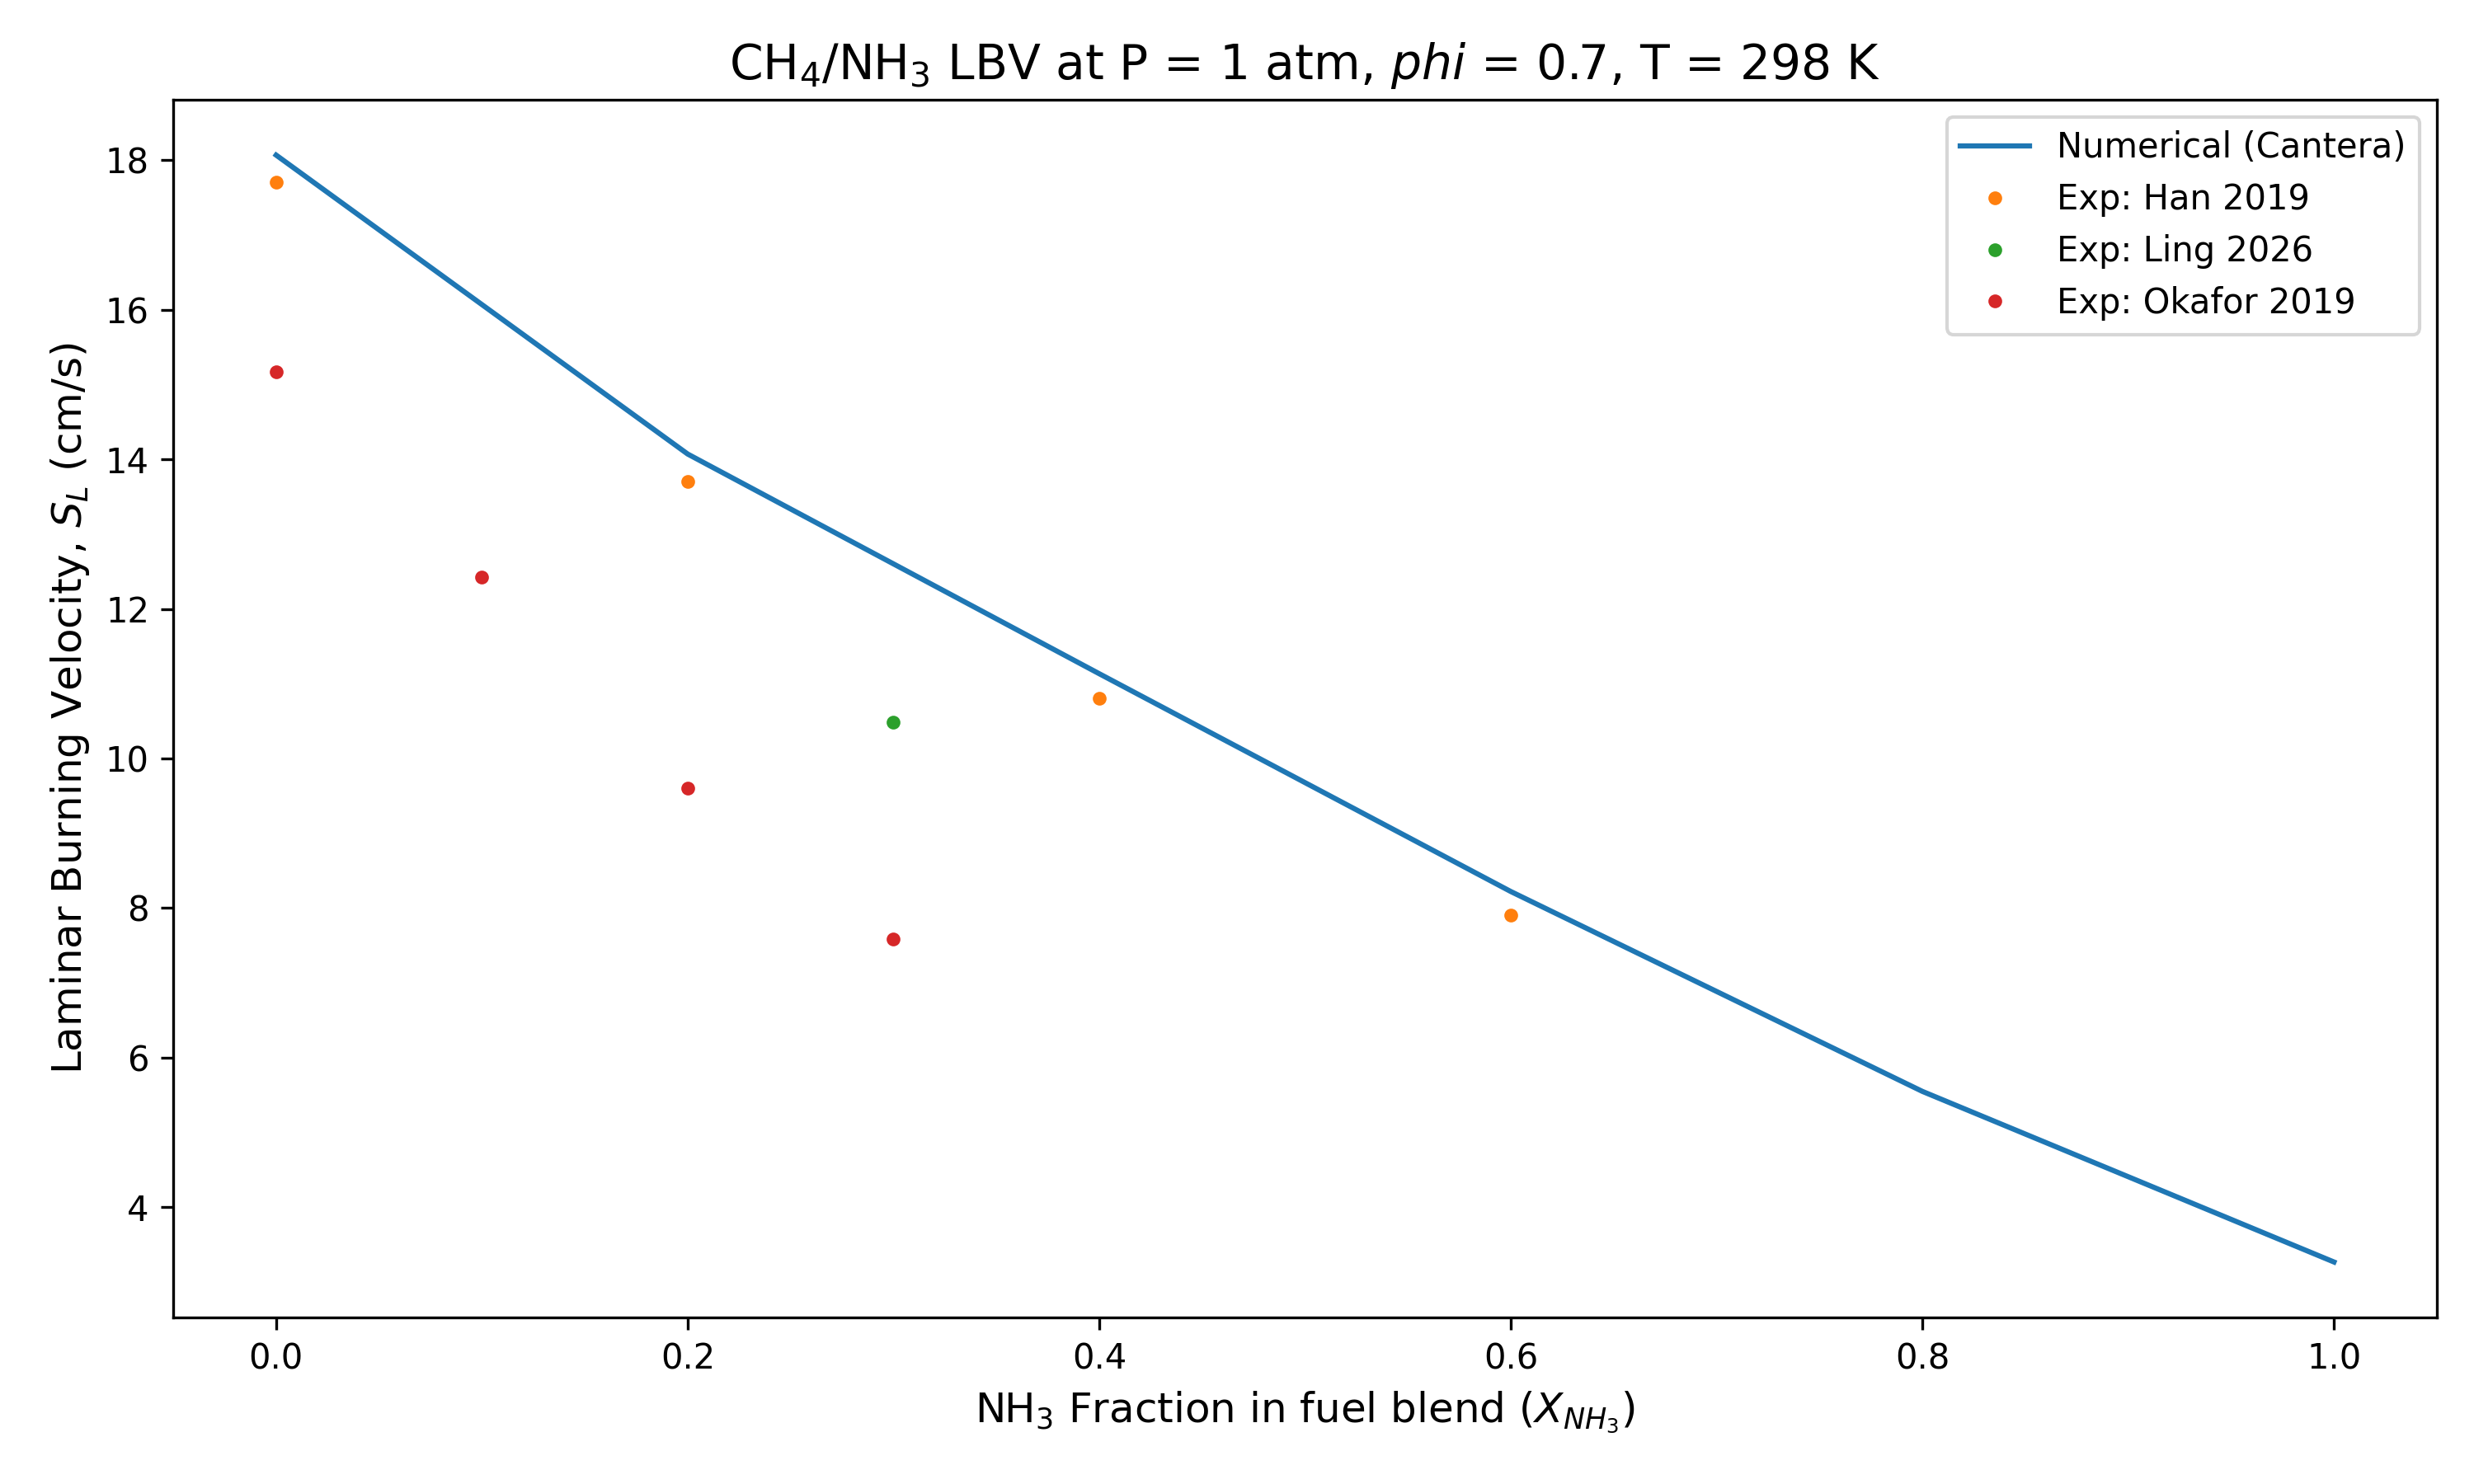
\includegraphics[width=\textwidth]{figures_ch4-nh3/lbv_p-1_phi-7.png}
			\caption{lean equivalence ratio}\label{}
		\end{subfigure}
		\hfill
		\begin{subfigure}[b]{0.45\textwidth}
			\centering
			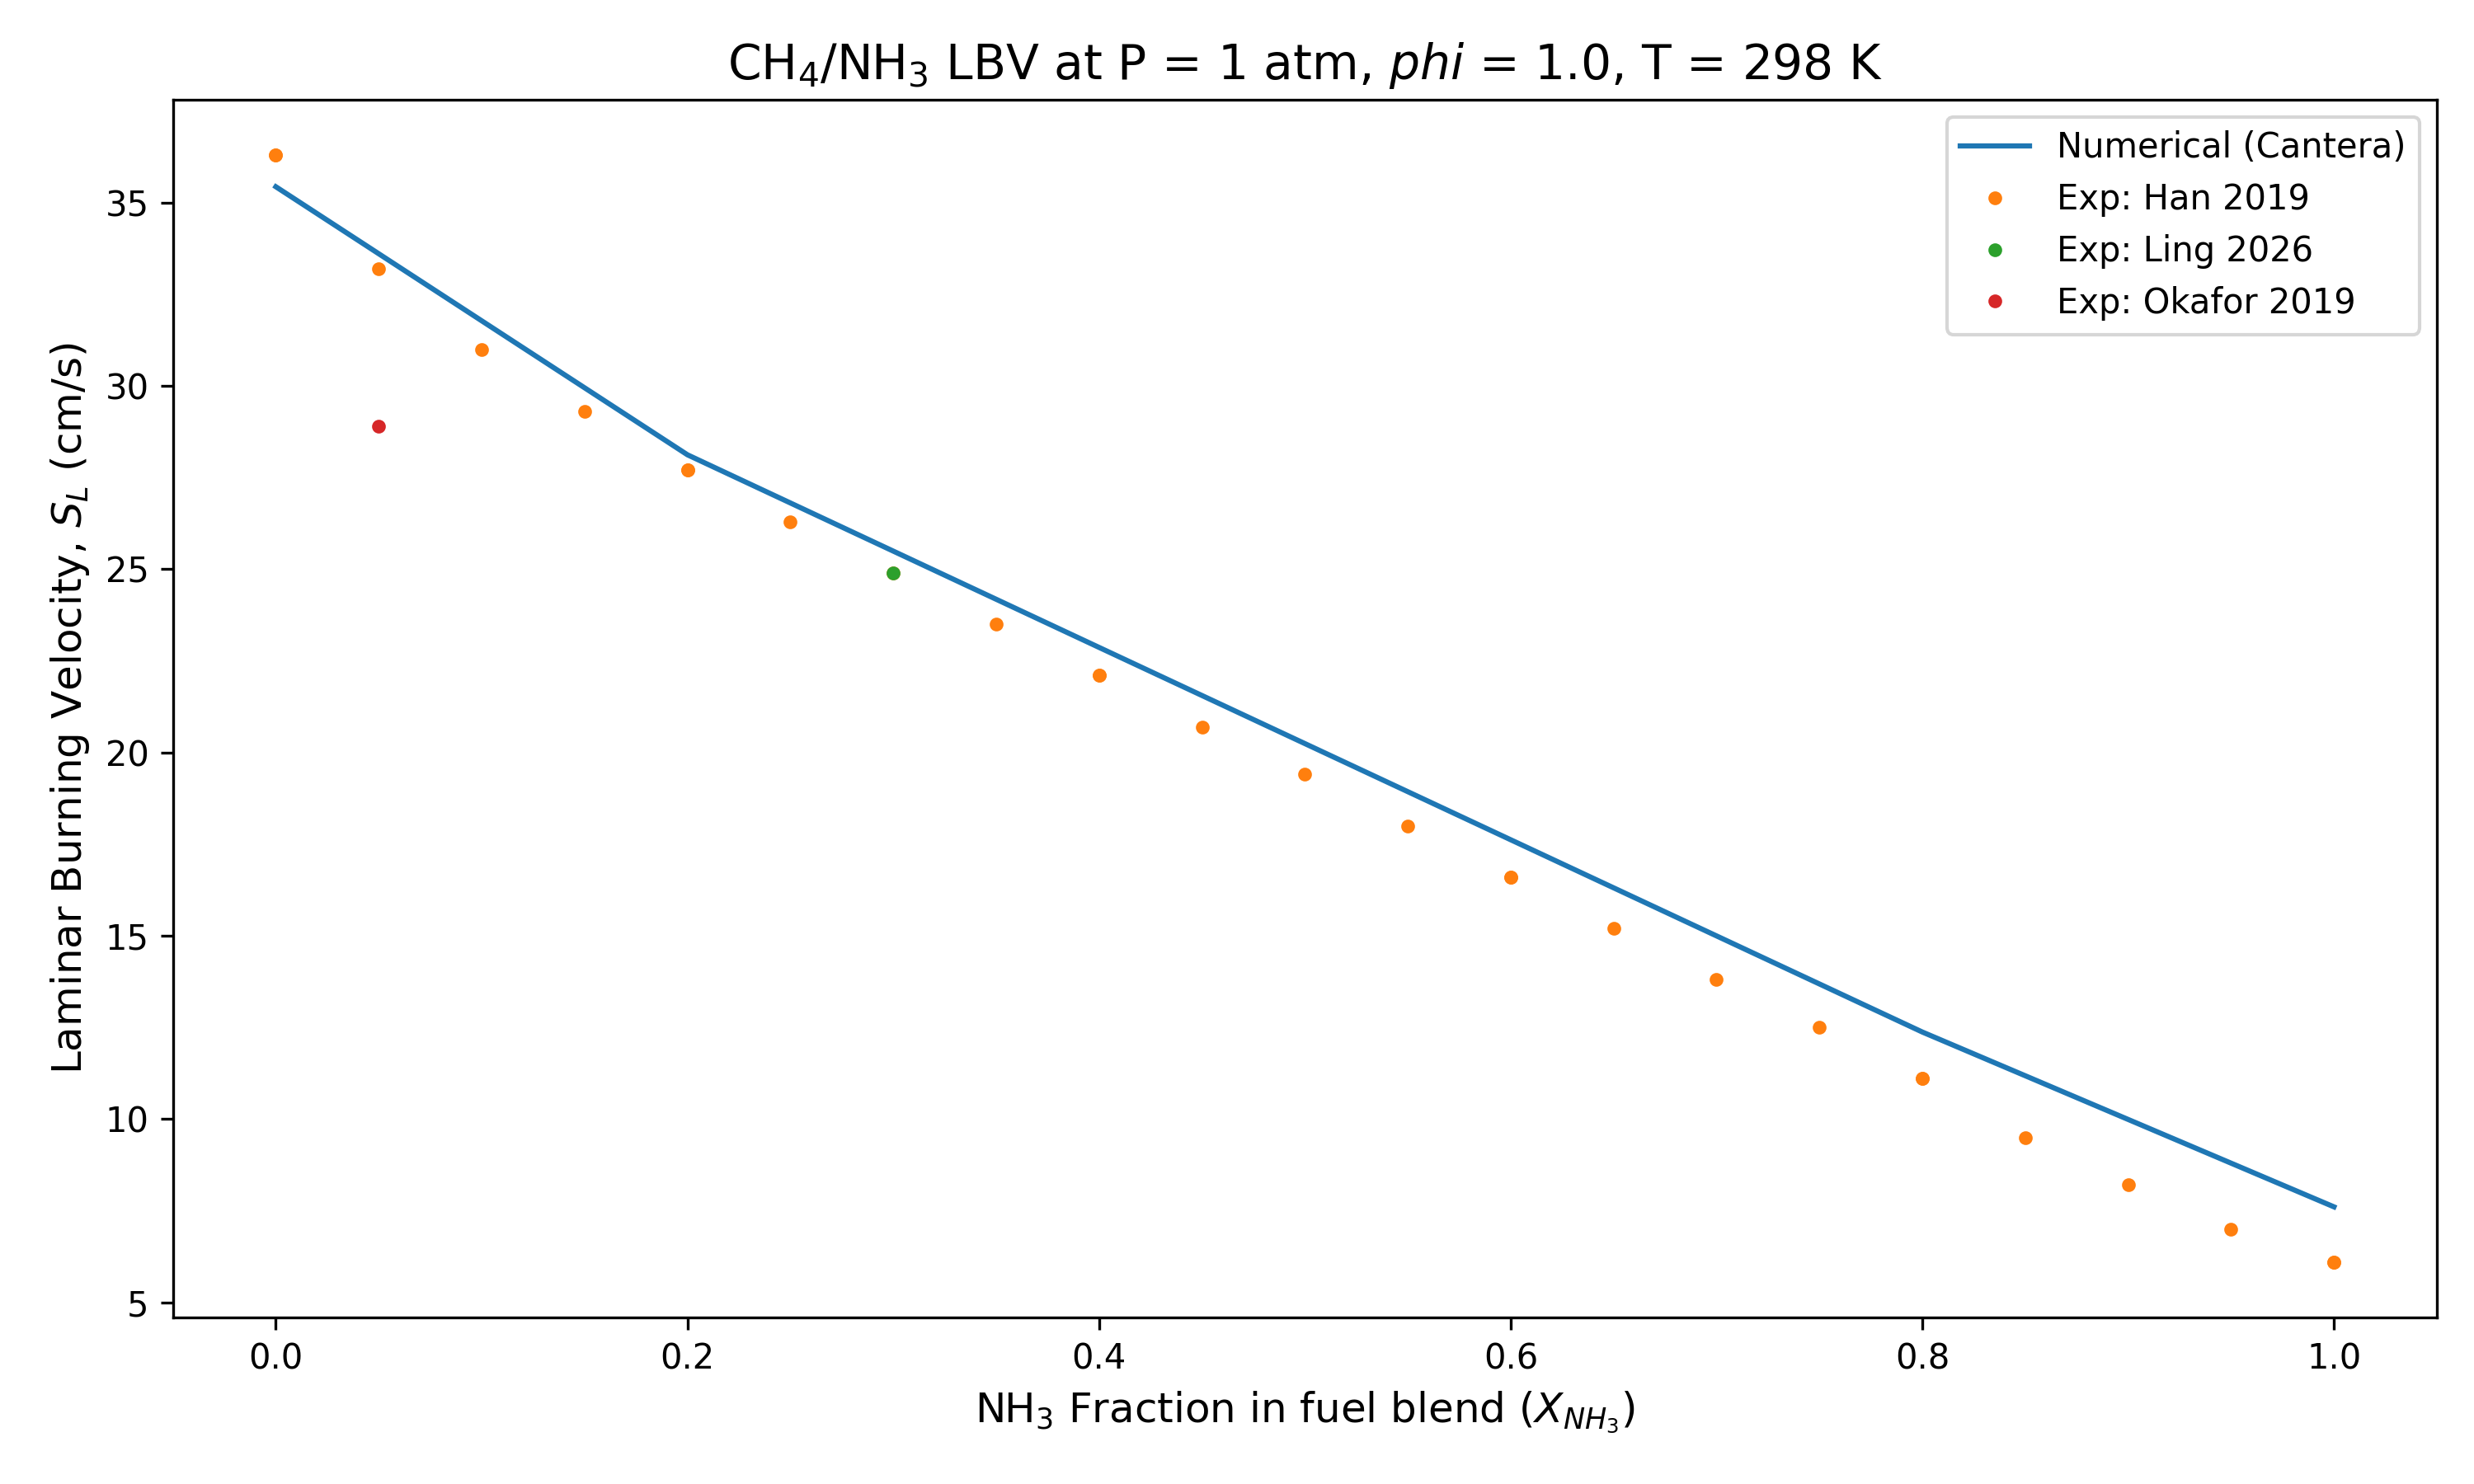
\includegraphics[width=\textwidth]{figures_ch4-nh3/lbv_p-1_phi-10.png}
			\caption{stoichiometric equivalence ratio}\label{}
		\end{subfigure}\\
		\begin{subfigure}[b]{0.45\textwidth}
			\centering
			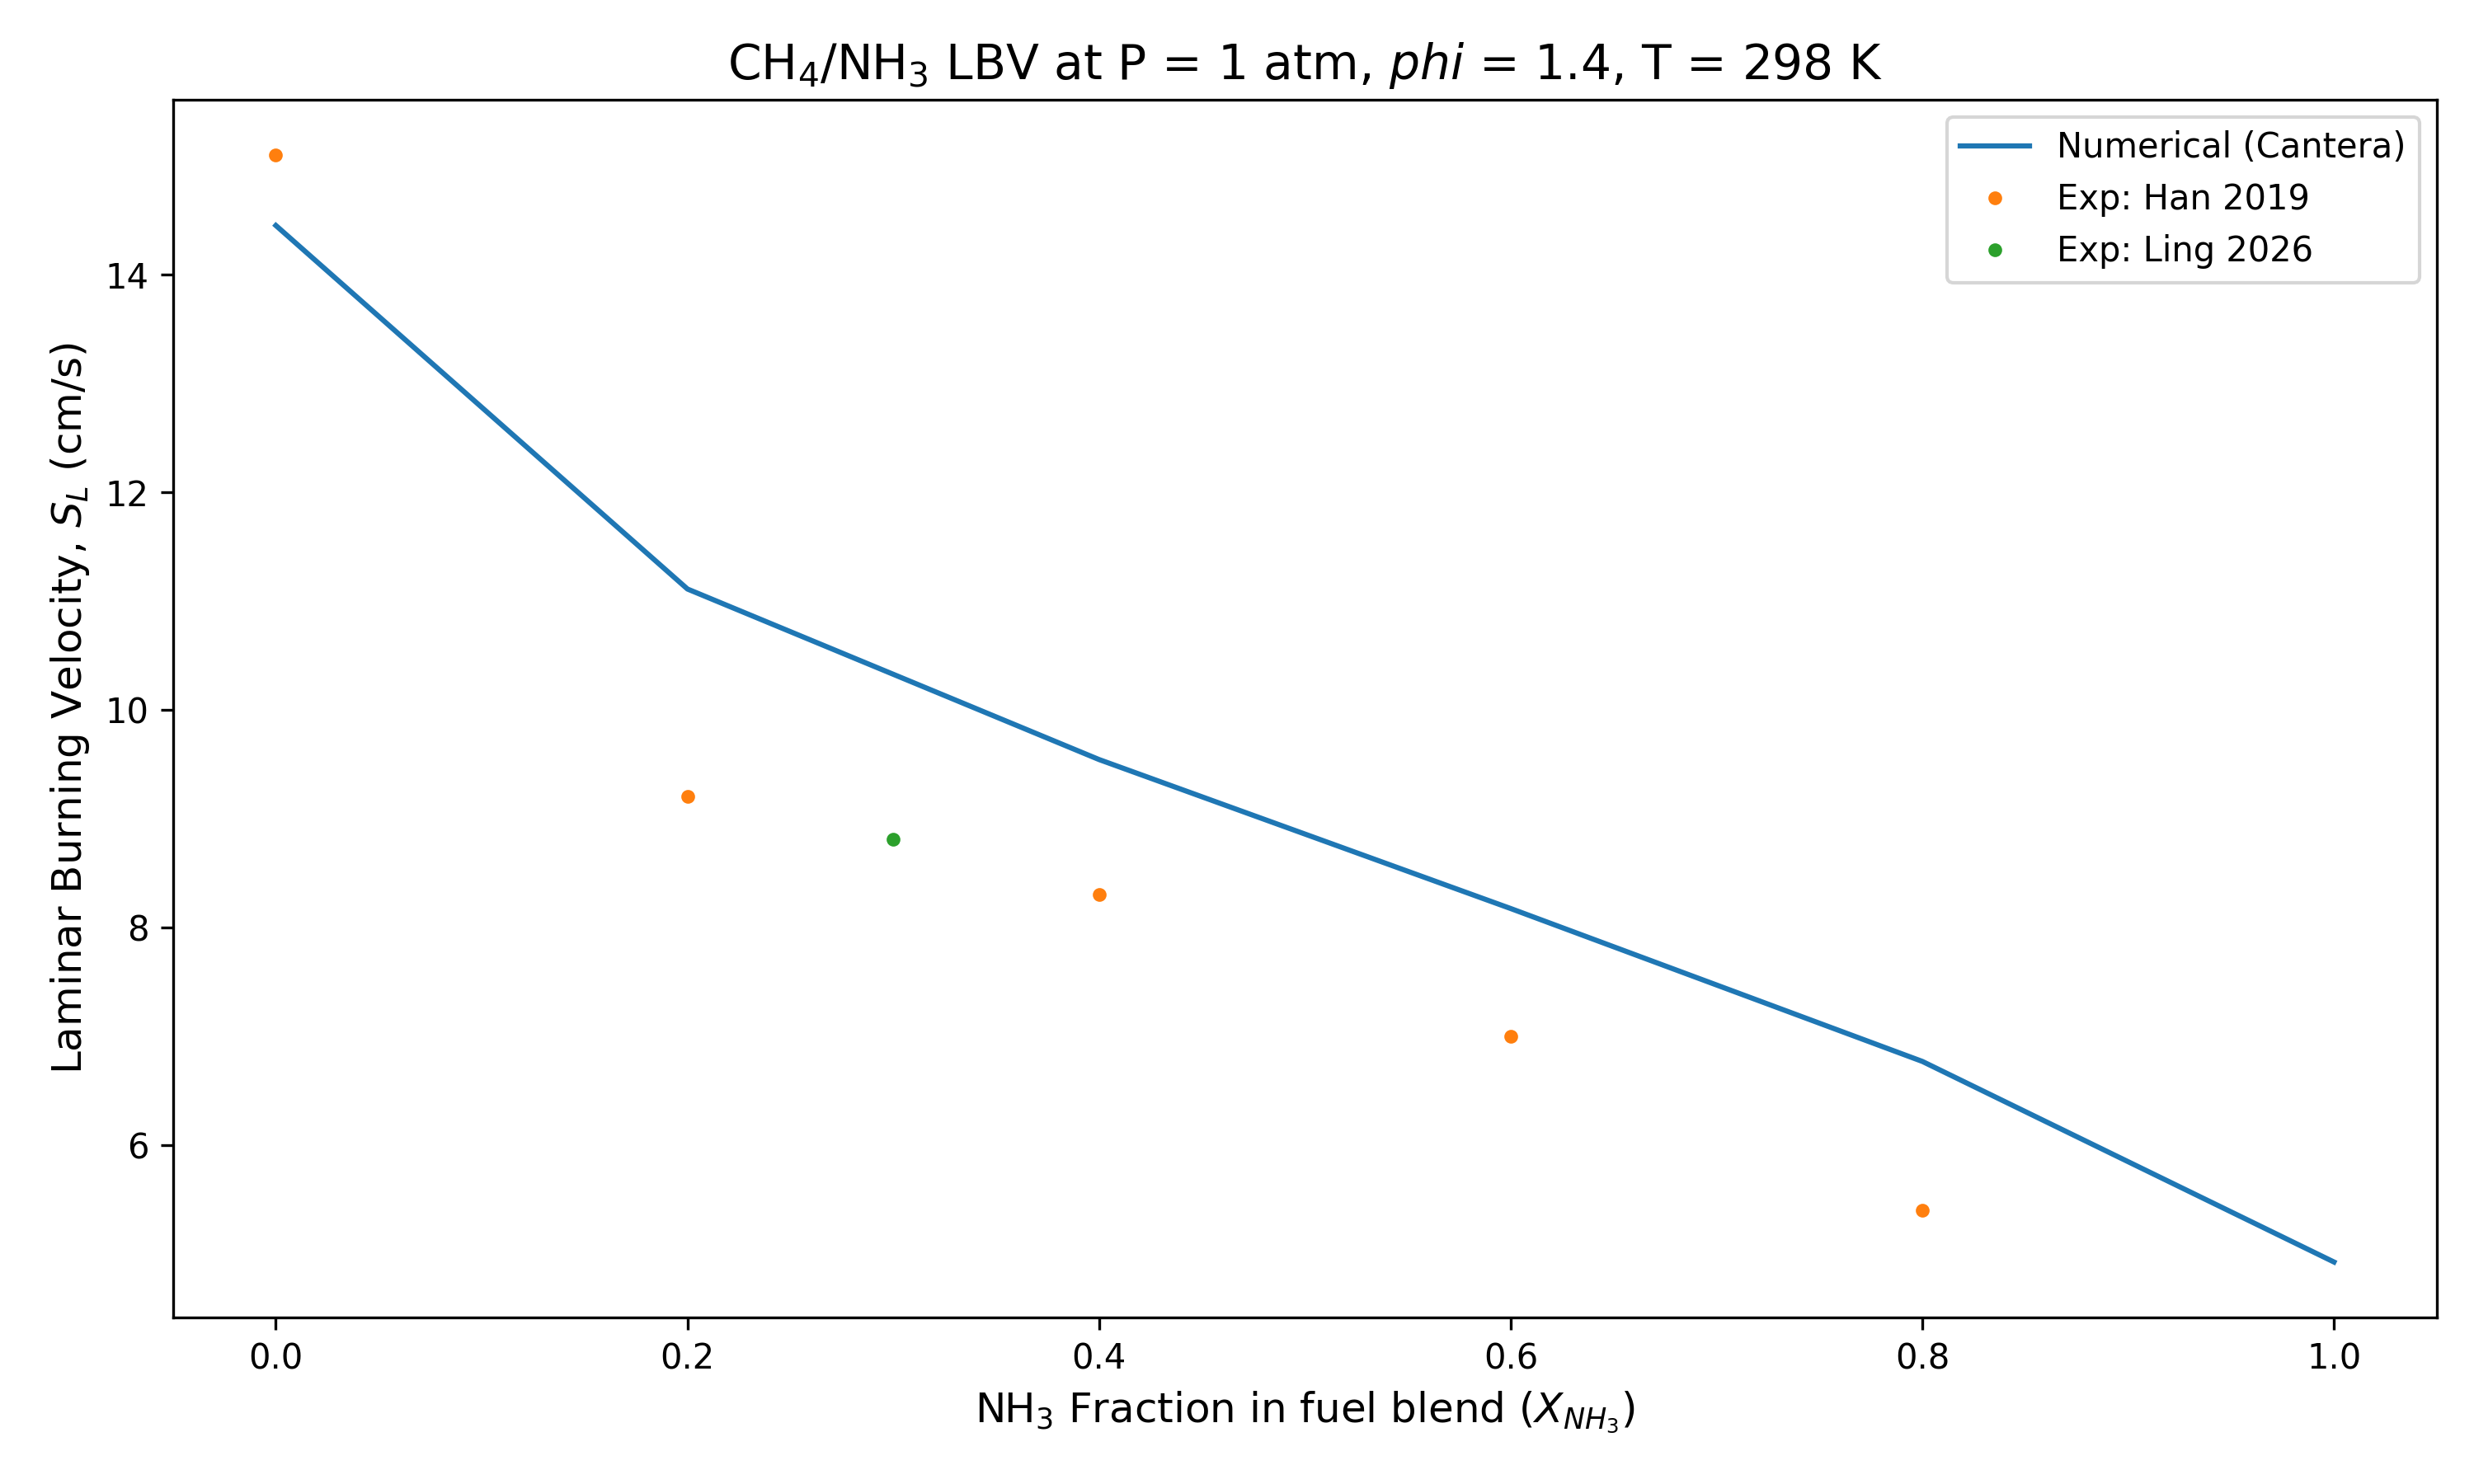
\includegraphics[width=\textwidth]{figures_ch4-nh3/lbv_p-1_phi-14.png}
			\caption{rich equivalence ratio}
			\label{}
		\end{subfigure}
	\end{figure}
\end{frame}

\begin{frame}{Validating Abe Mechanism}
	Laminar burning velocity of CH$_4$/NH$_3$/Air flame at 3atm of pressure
	\begin{figure}[htbp]
		\centering
		\begin{subfigure}[b]{0.45\textwidth}
			\centering
			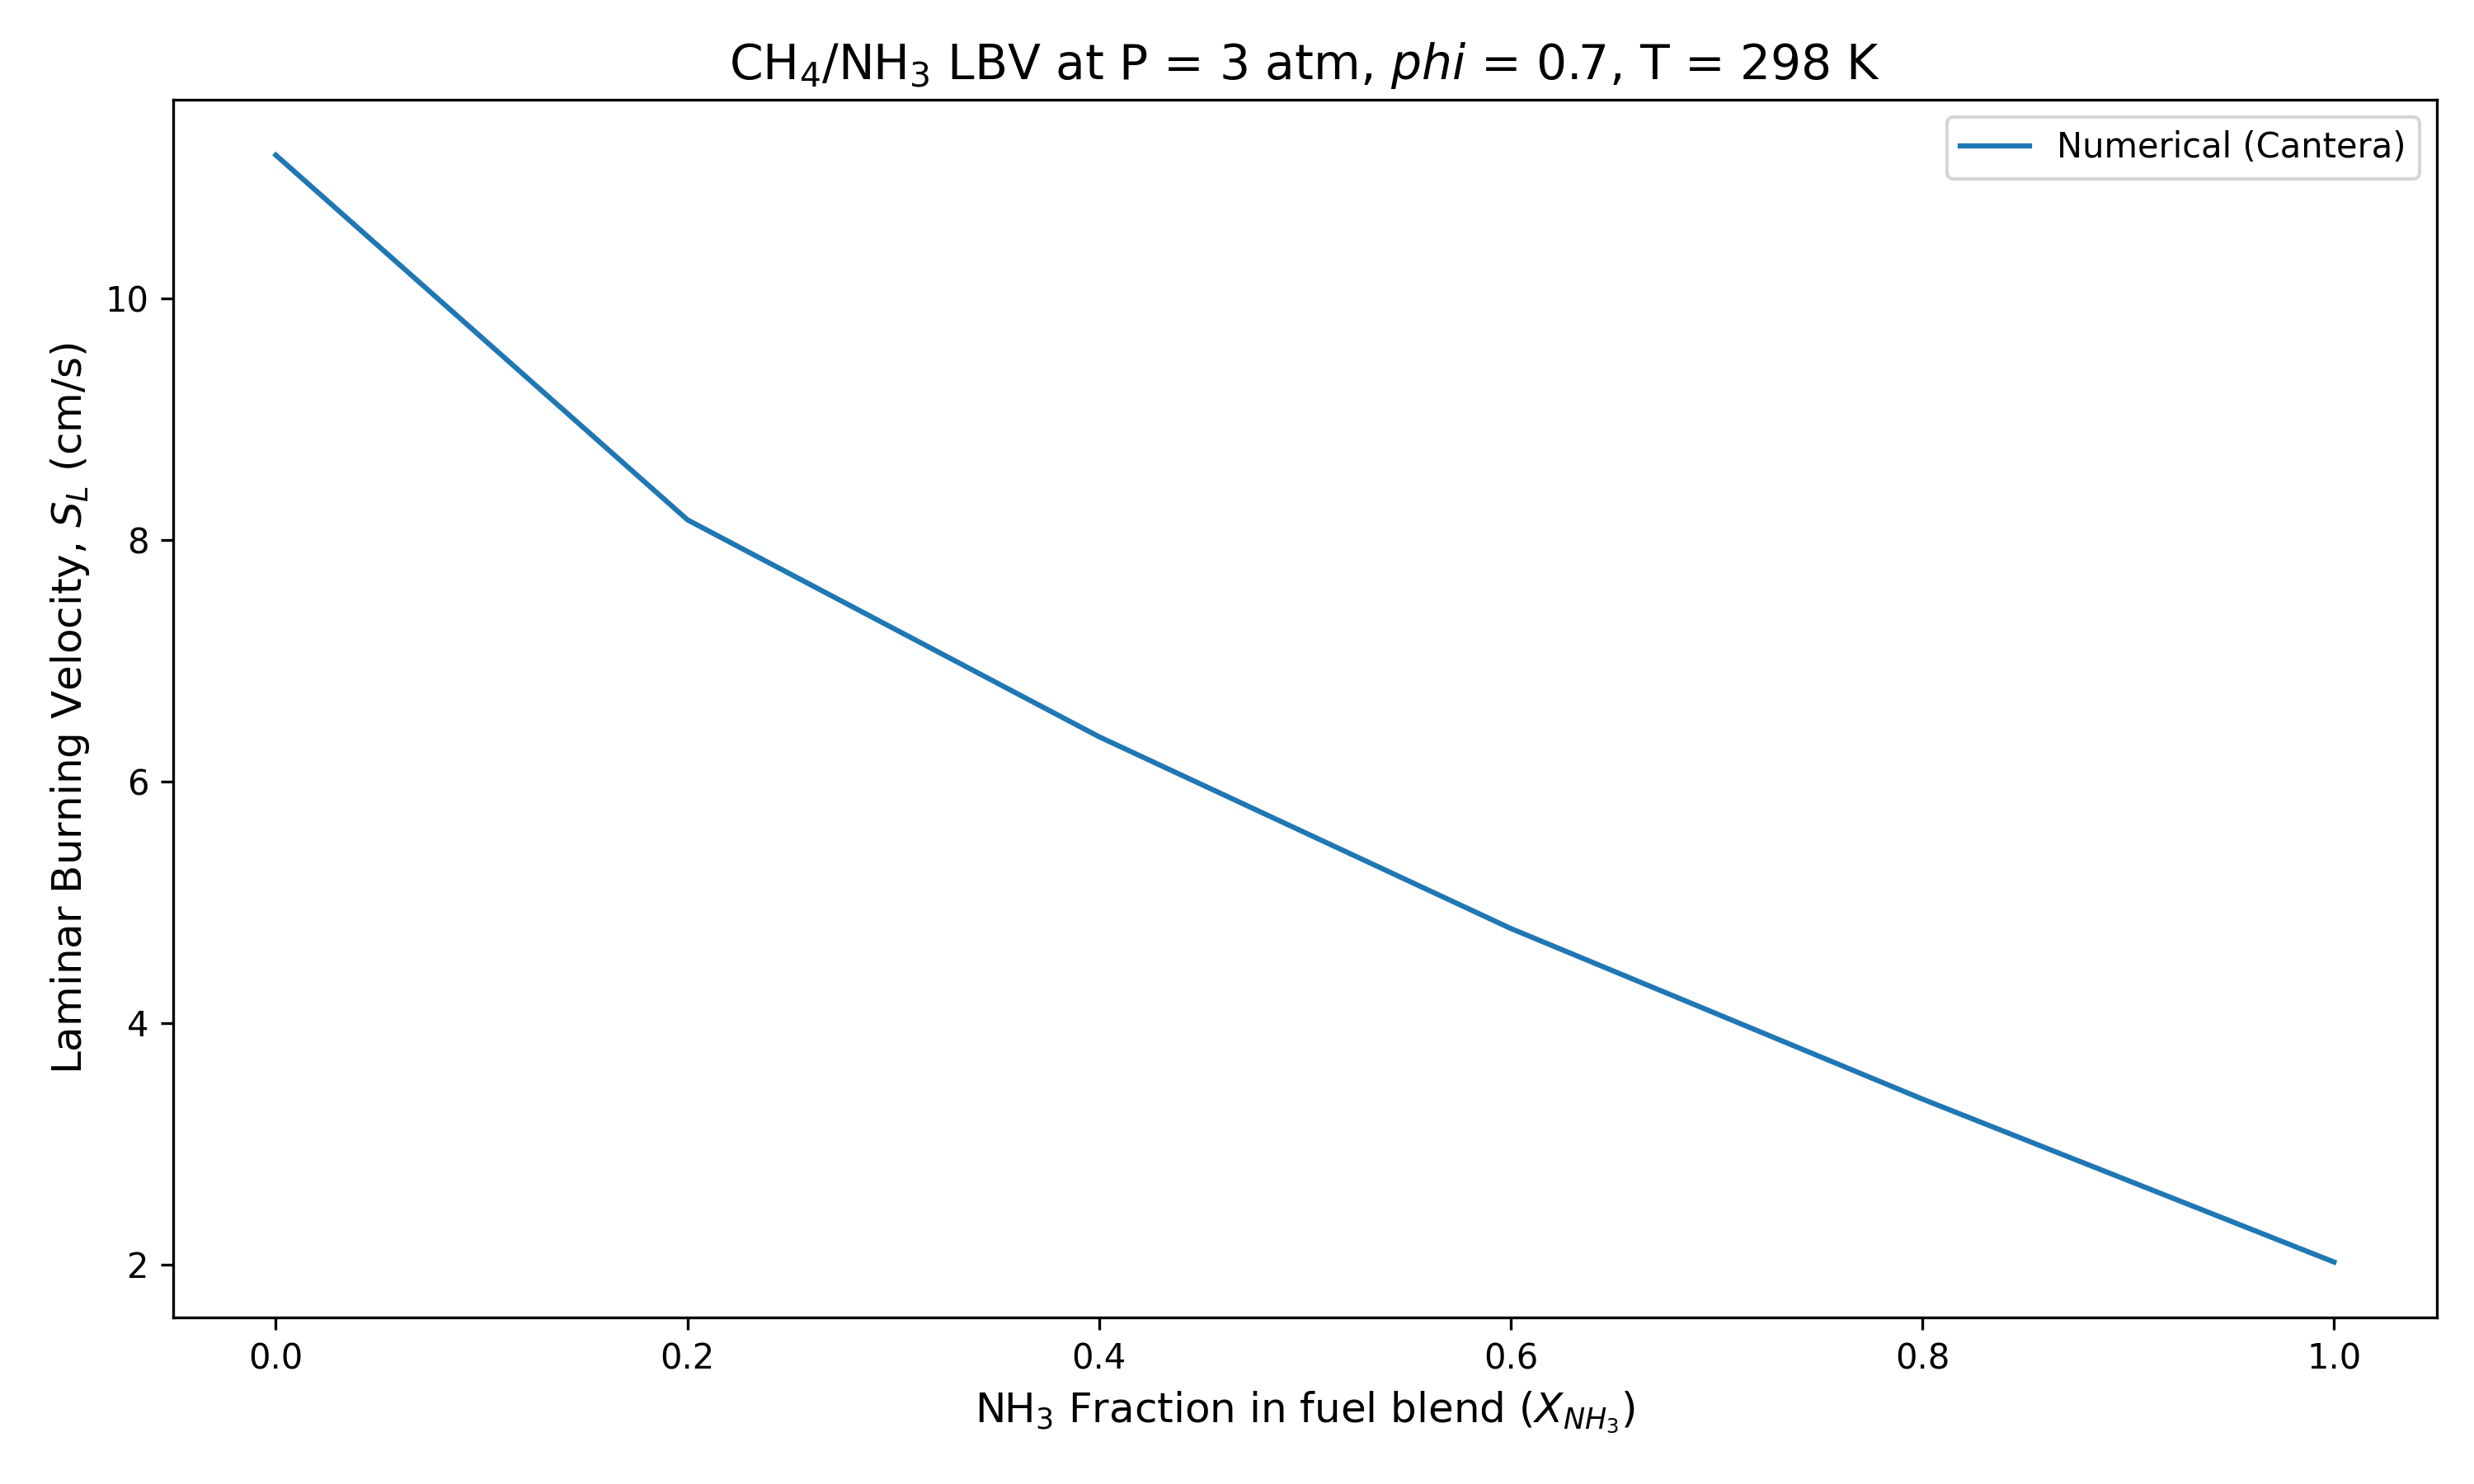
\includegraphics[width=\textwidth]{figures_ch4-nh3/lbv_p-3_phi-7.png}
			\caption{lean equivalence ratio}\label{}
		\end{subfigure}
		\hfill
		\begin{subfigure}[b]{0.45\textwidth}
			\centering
			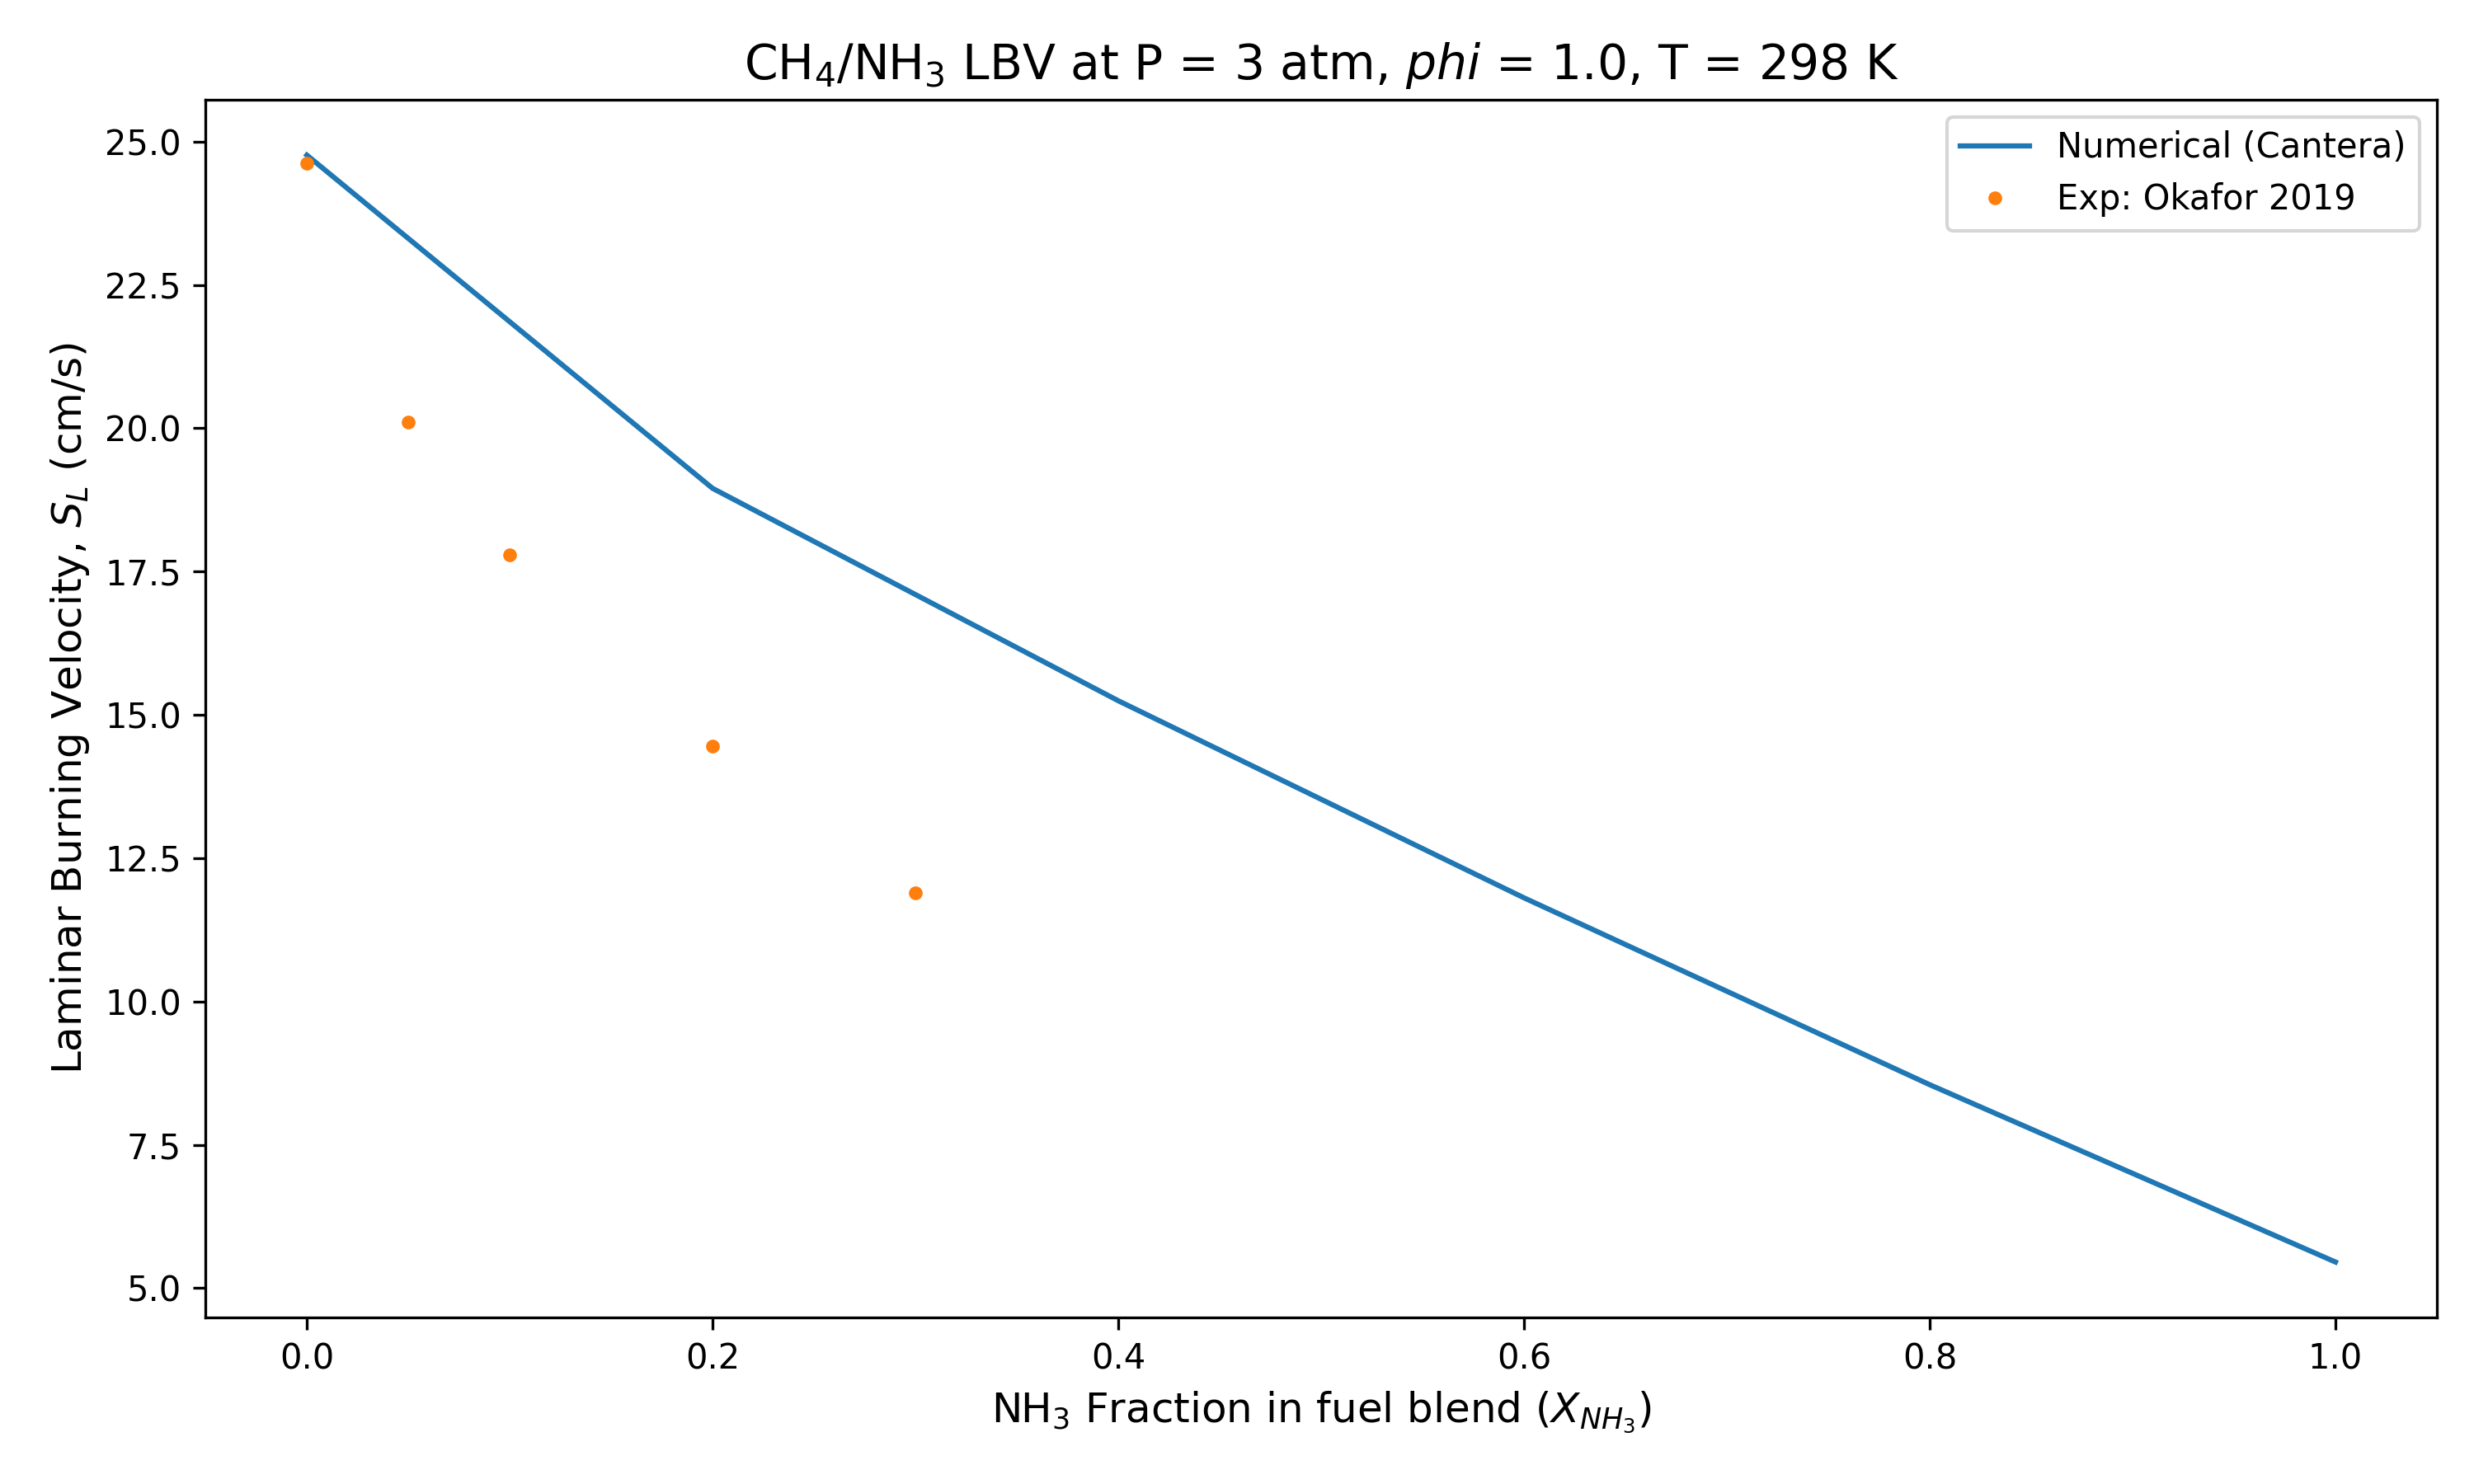
\includegraphics[width=\textwidth]{figures_ch4-nh3/lbv_p-3_phi-10.png}
			\caption{stoichiometric equivalence ratio}\label{}
		\end{subfigure}\\
		\begin{subfigure}[b]{0.45\textwidth}
			\centering
			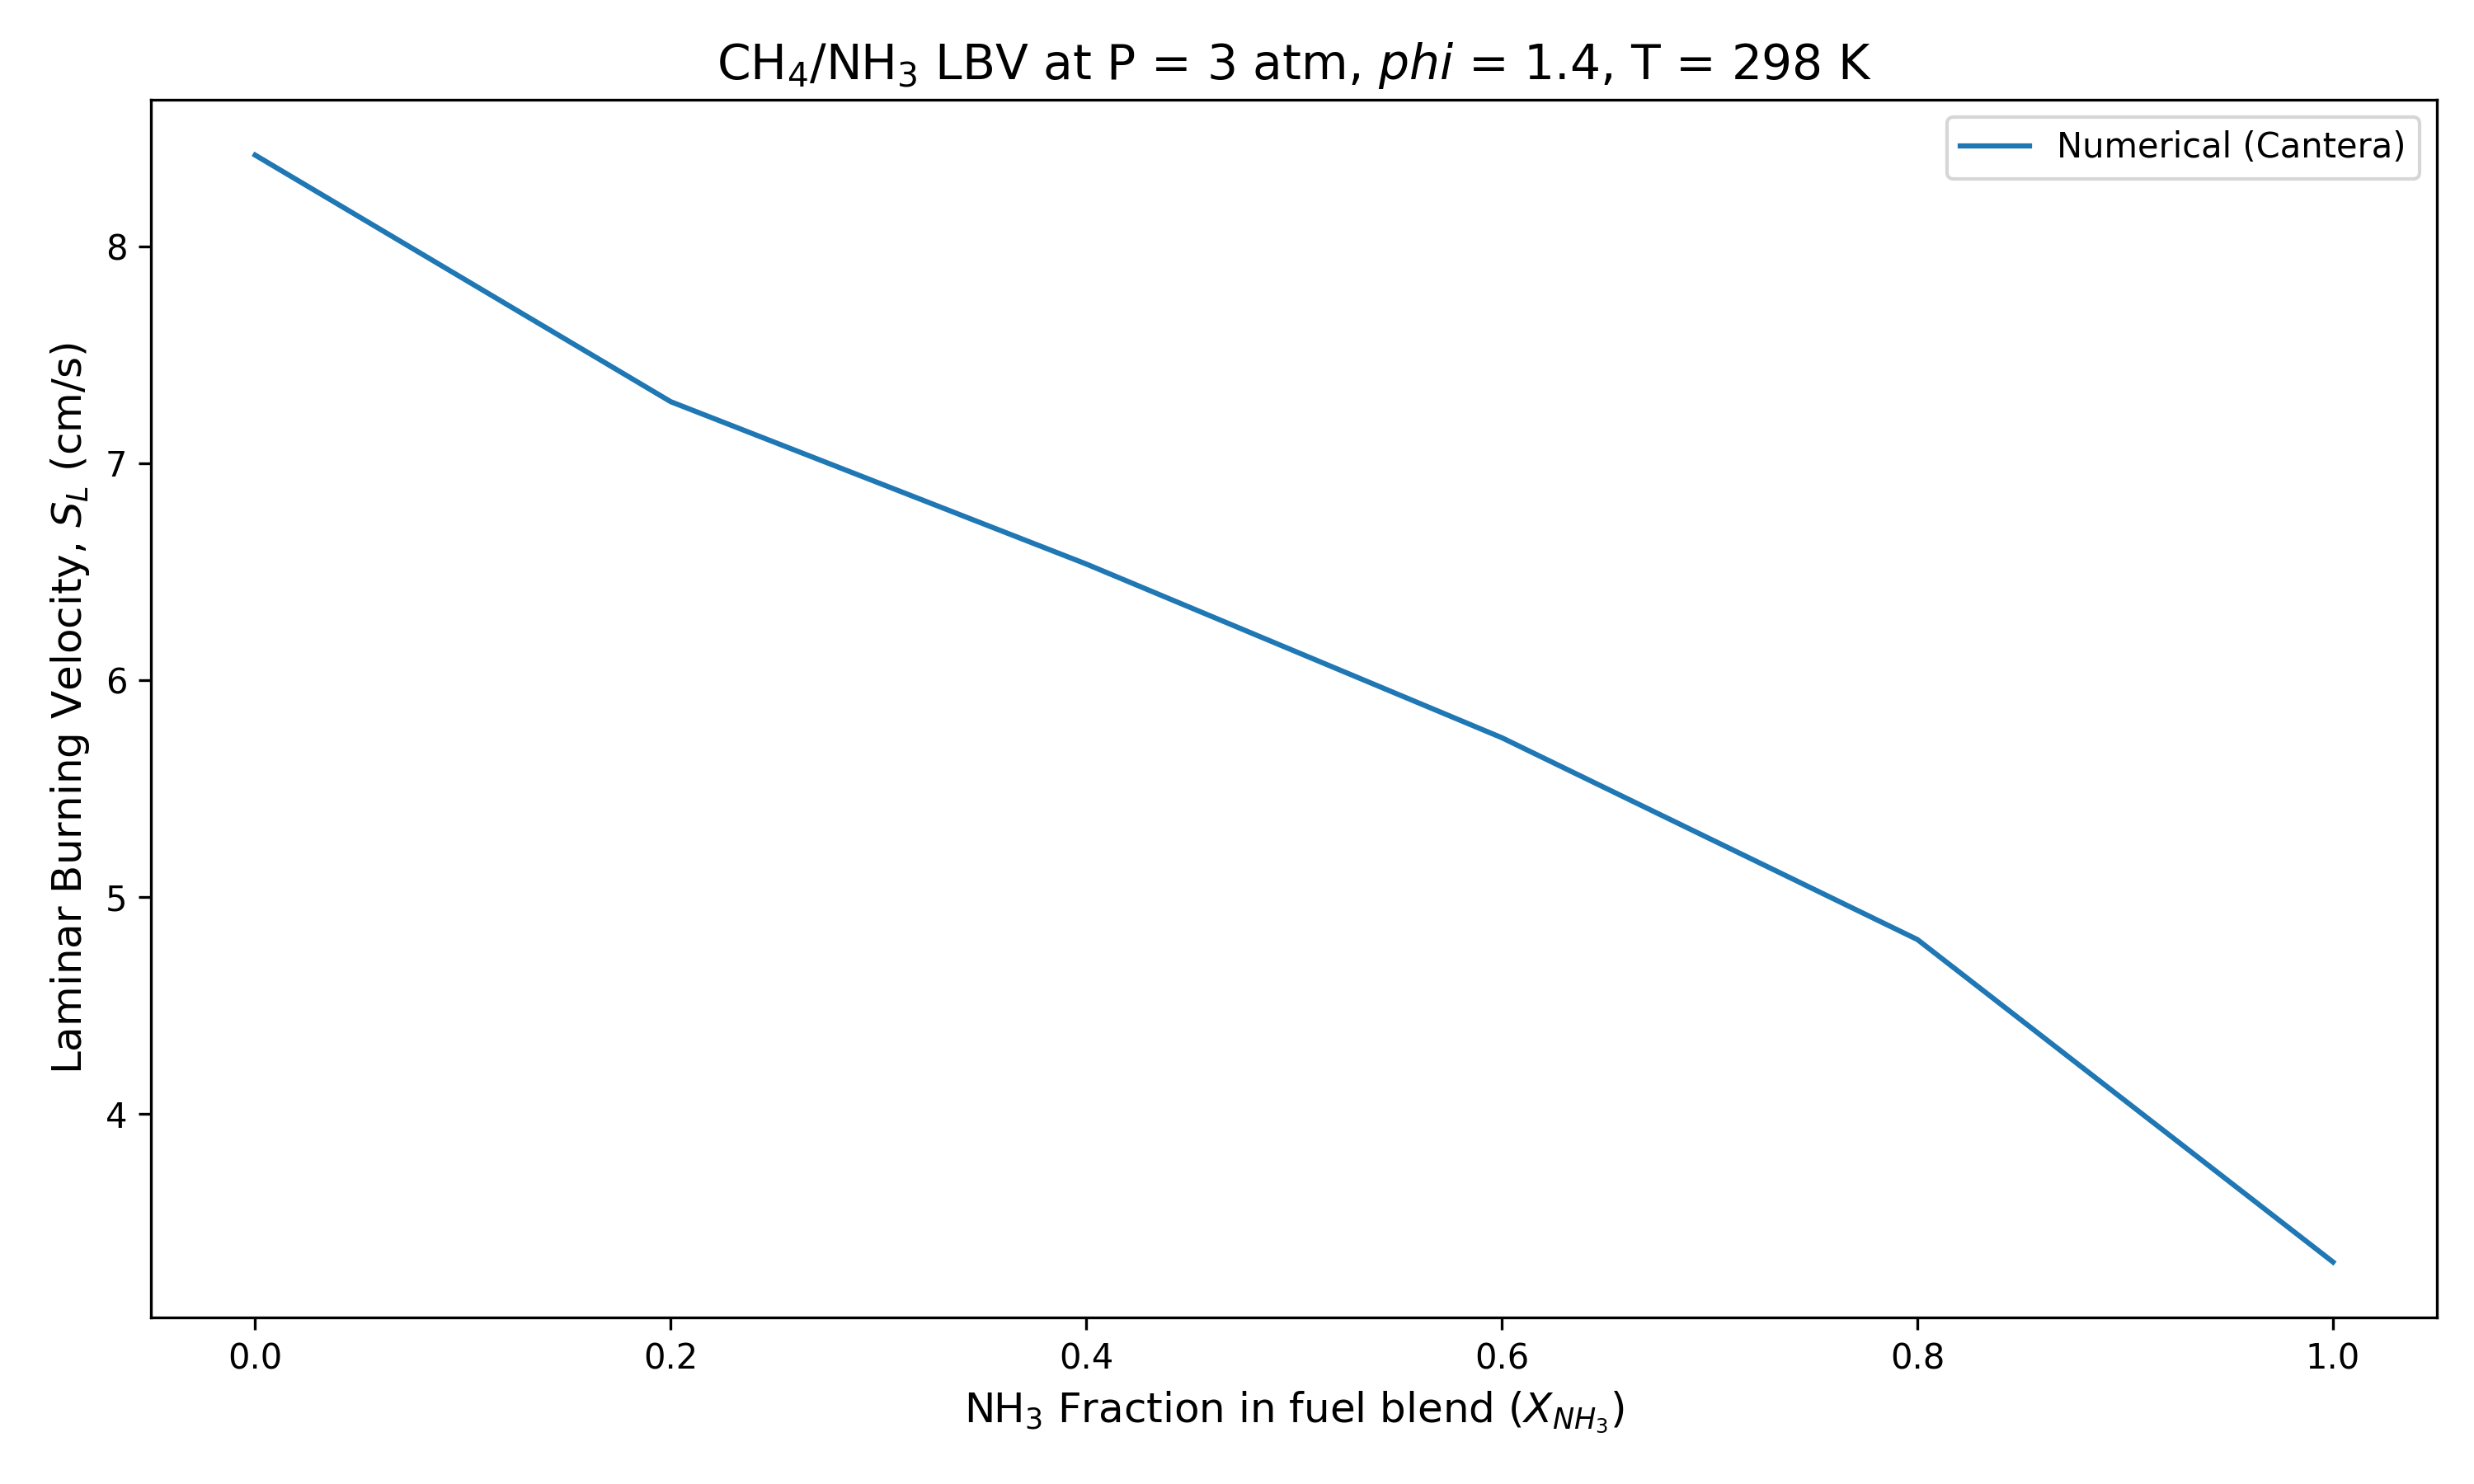
\includegraphics[width=\textwidth]{figures_ch4-nh3/lbv_p-3_phi-14.png}
			\caption{rich equivalence ratio}
			\label{}
		\end{subfigure}
	\end{figure}
\end{frame}

\begin{frame}{Validating Abe Mechanism}
	Laminar burning velocity of CH$_4$/NH$_3$/Air flame at 5atm of pressure
	\begin{figure}[htbp]
		\centering
		\begin{subfigure}[b]{0.45\textwidth}
			\centering
			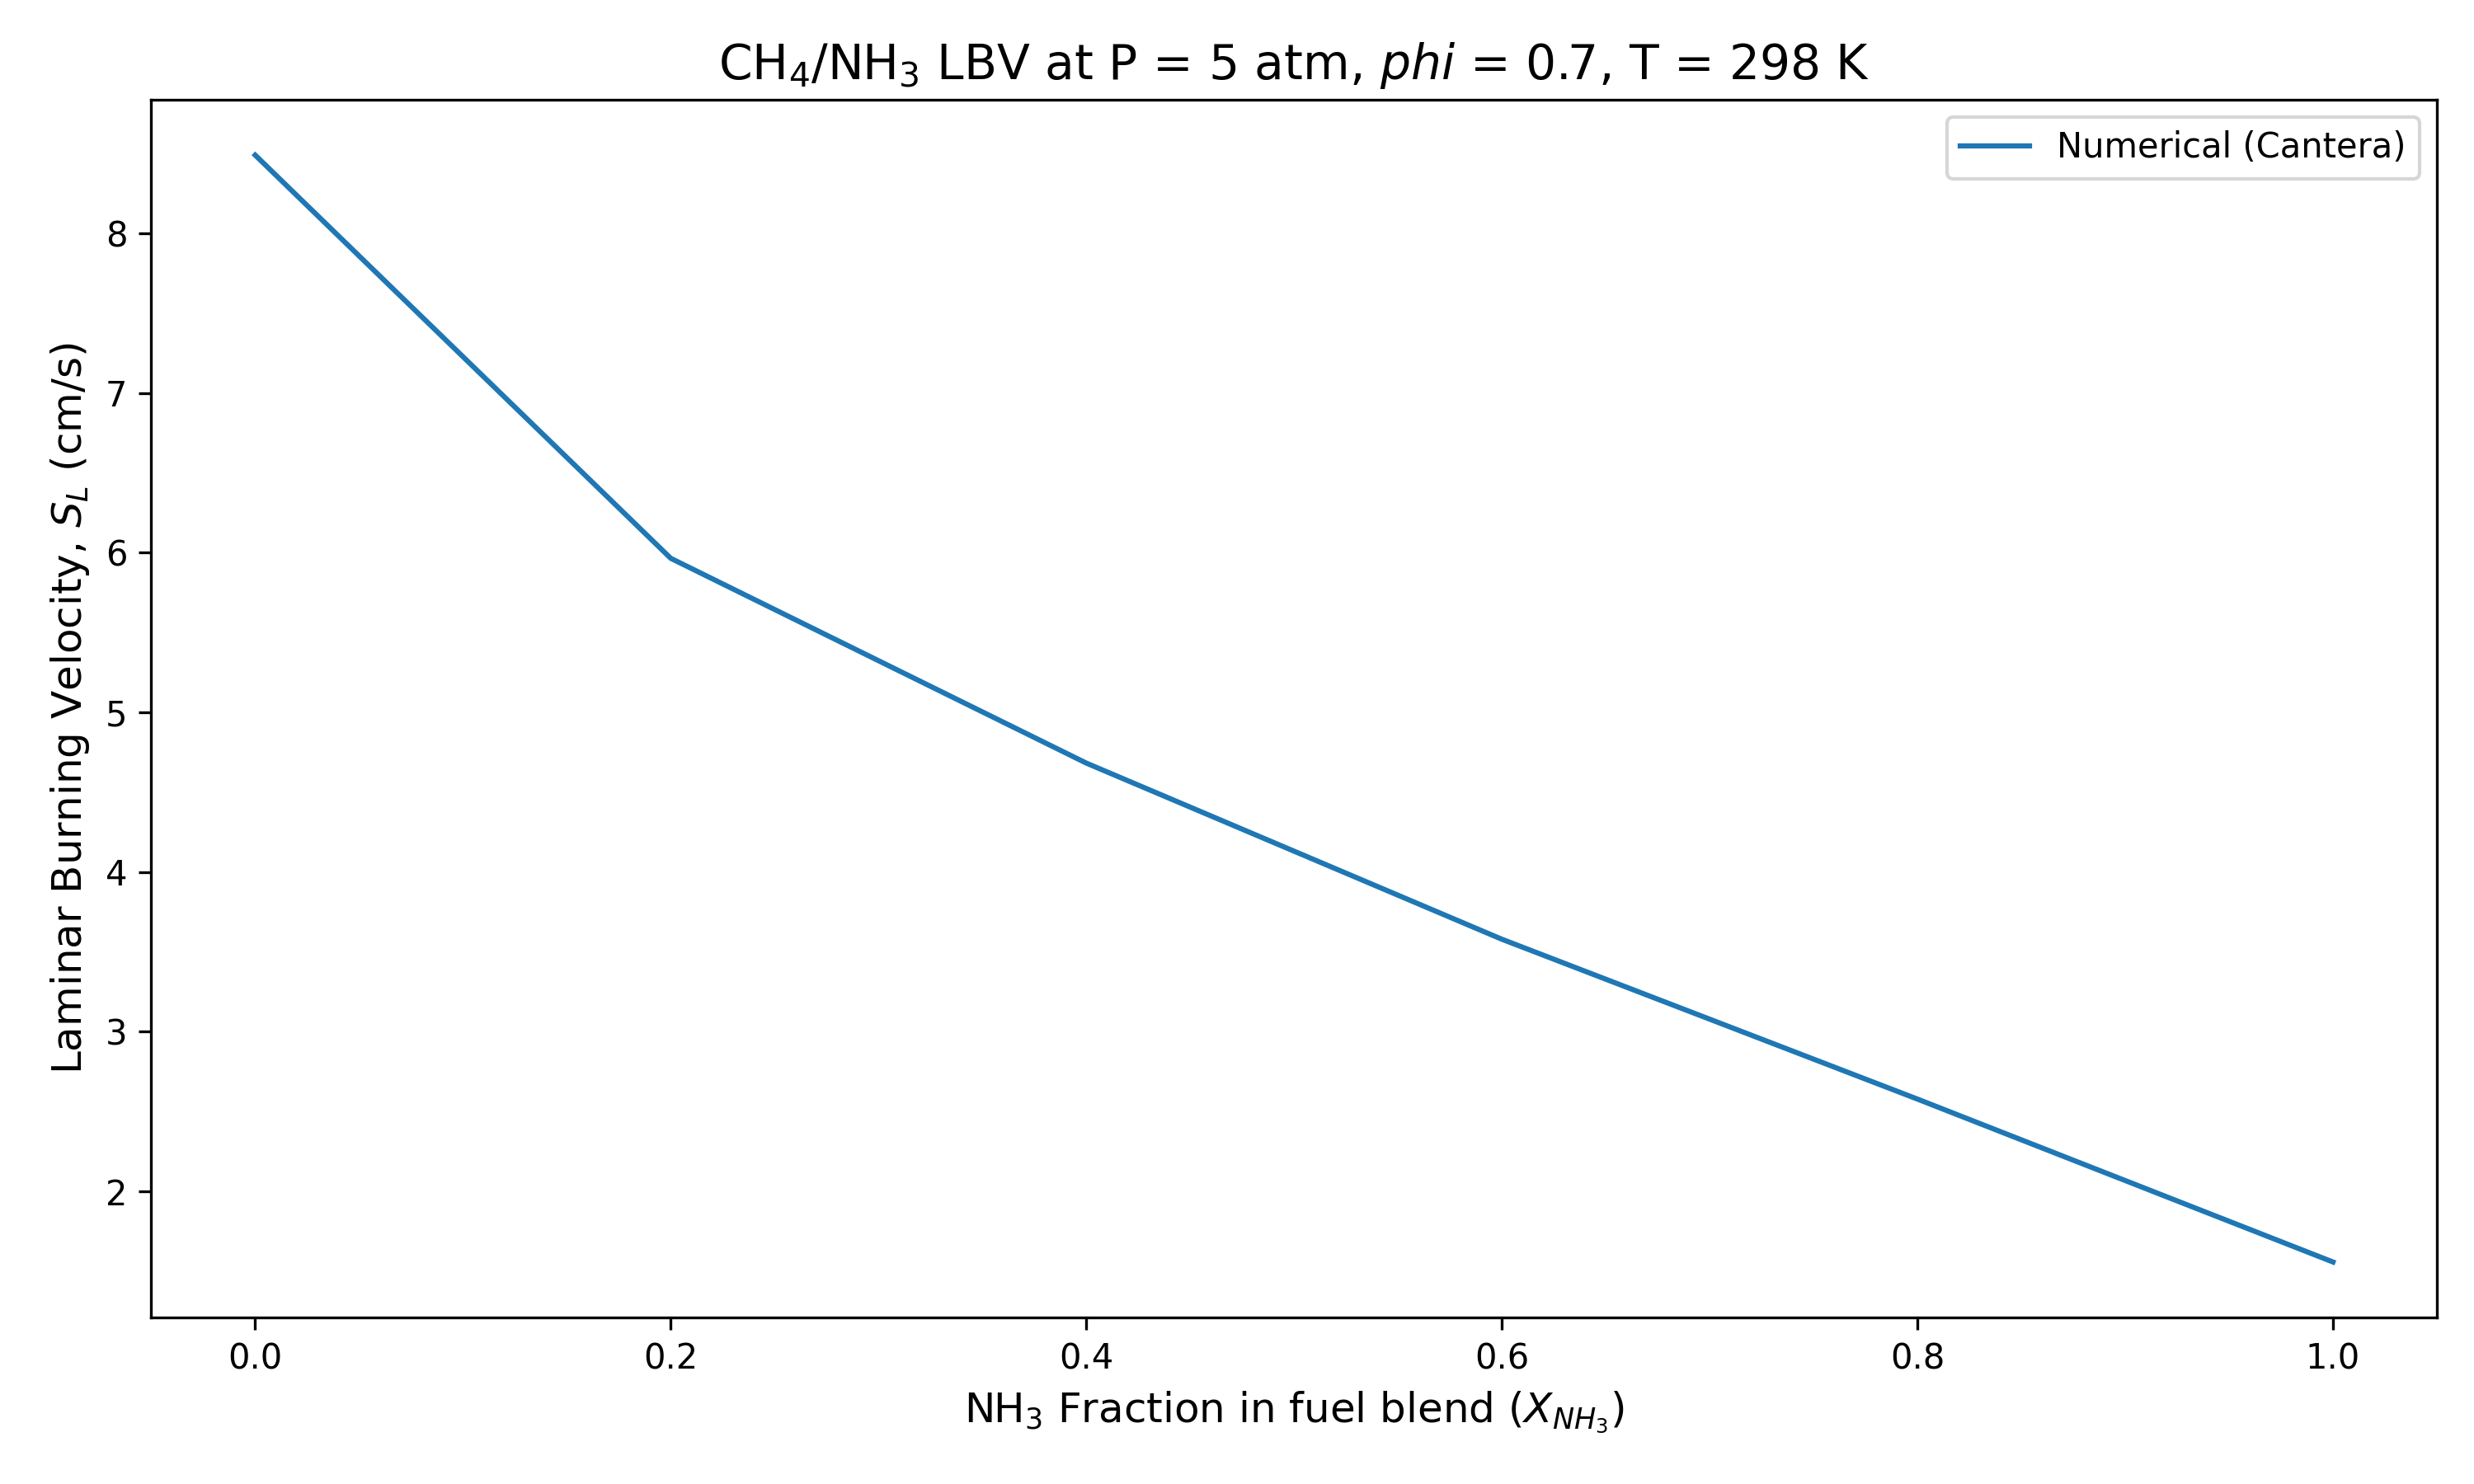
\includegraphics[width=\textwidth]{figures_ch4-nh3/lbv_p-5_phi-7.png}
			\caption{lean equivalence ratio}\label{}
		\end{subfigure}
		\hfill
		\begin{subfigure}[b]{0.45\textwidth}
			\centering
			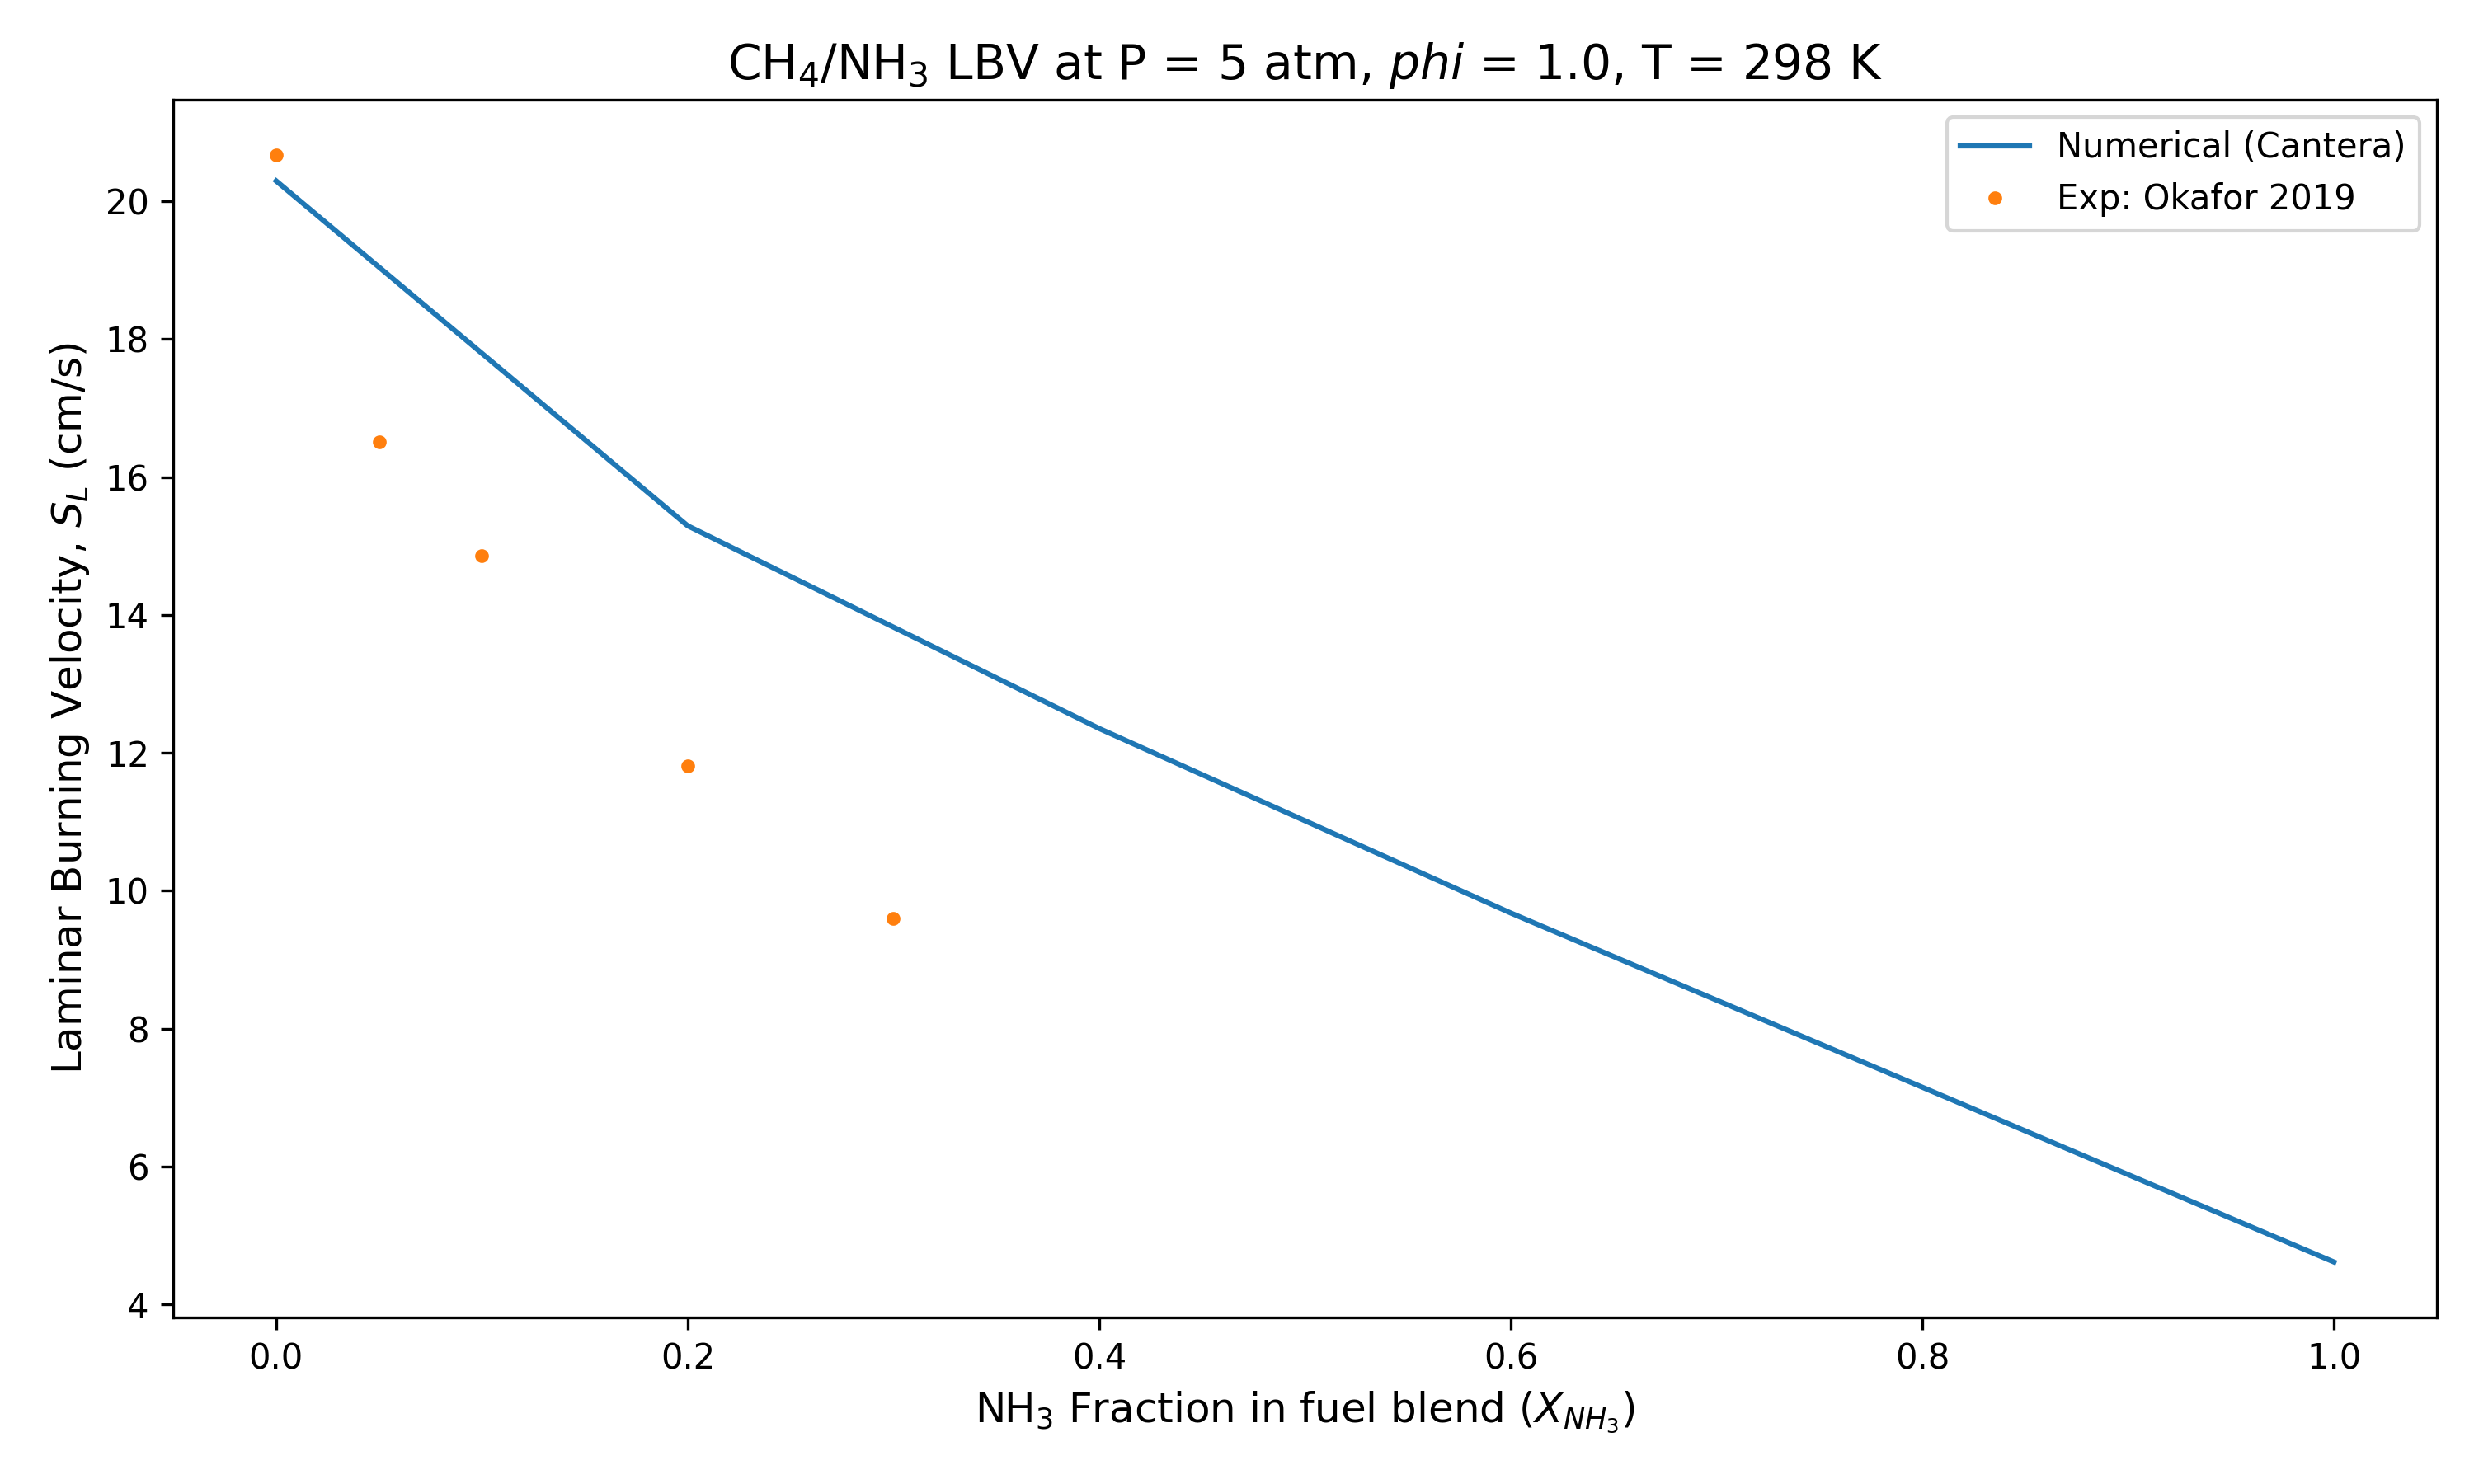
\includegraphics[width=\textwidth]{figures_ch4-nh3/lbv_p-5_phi-10.png}
			\caption{stoichiometric equivalence ratio}\label{}
		\end{subfigure}\\
		\begin{subfigure}[b]{0.45\textwidth}
			\centering
			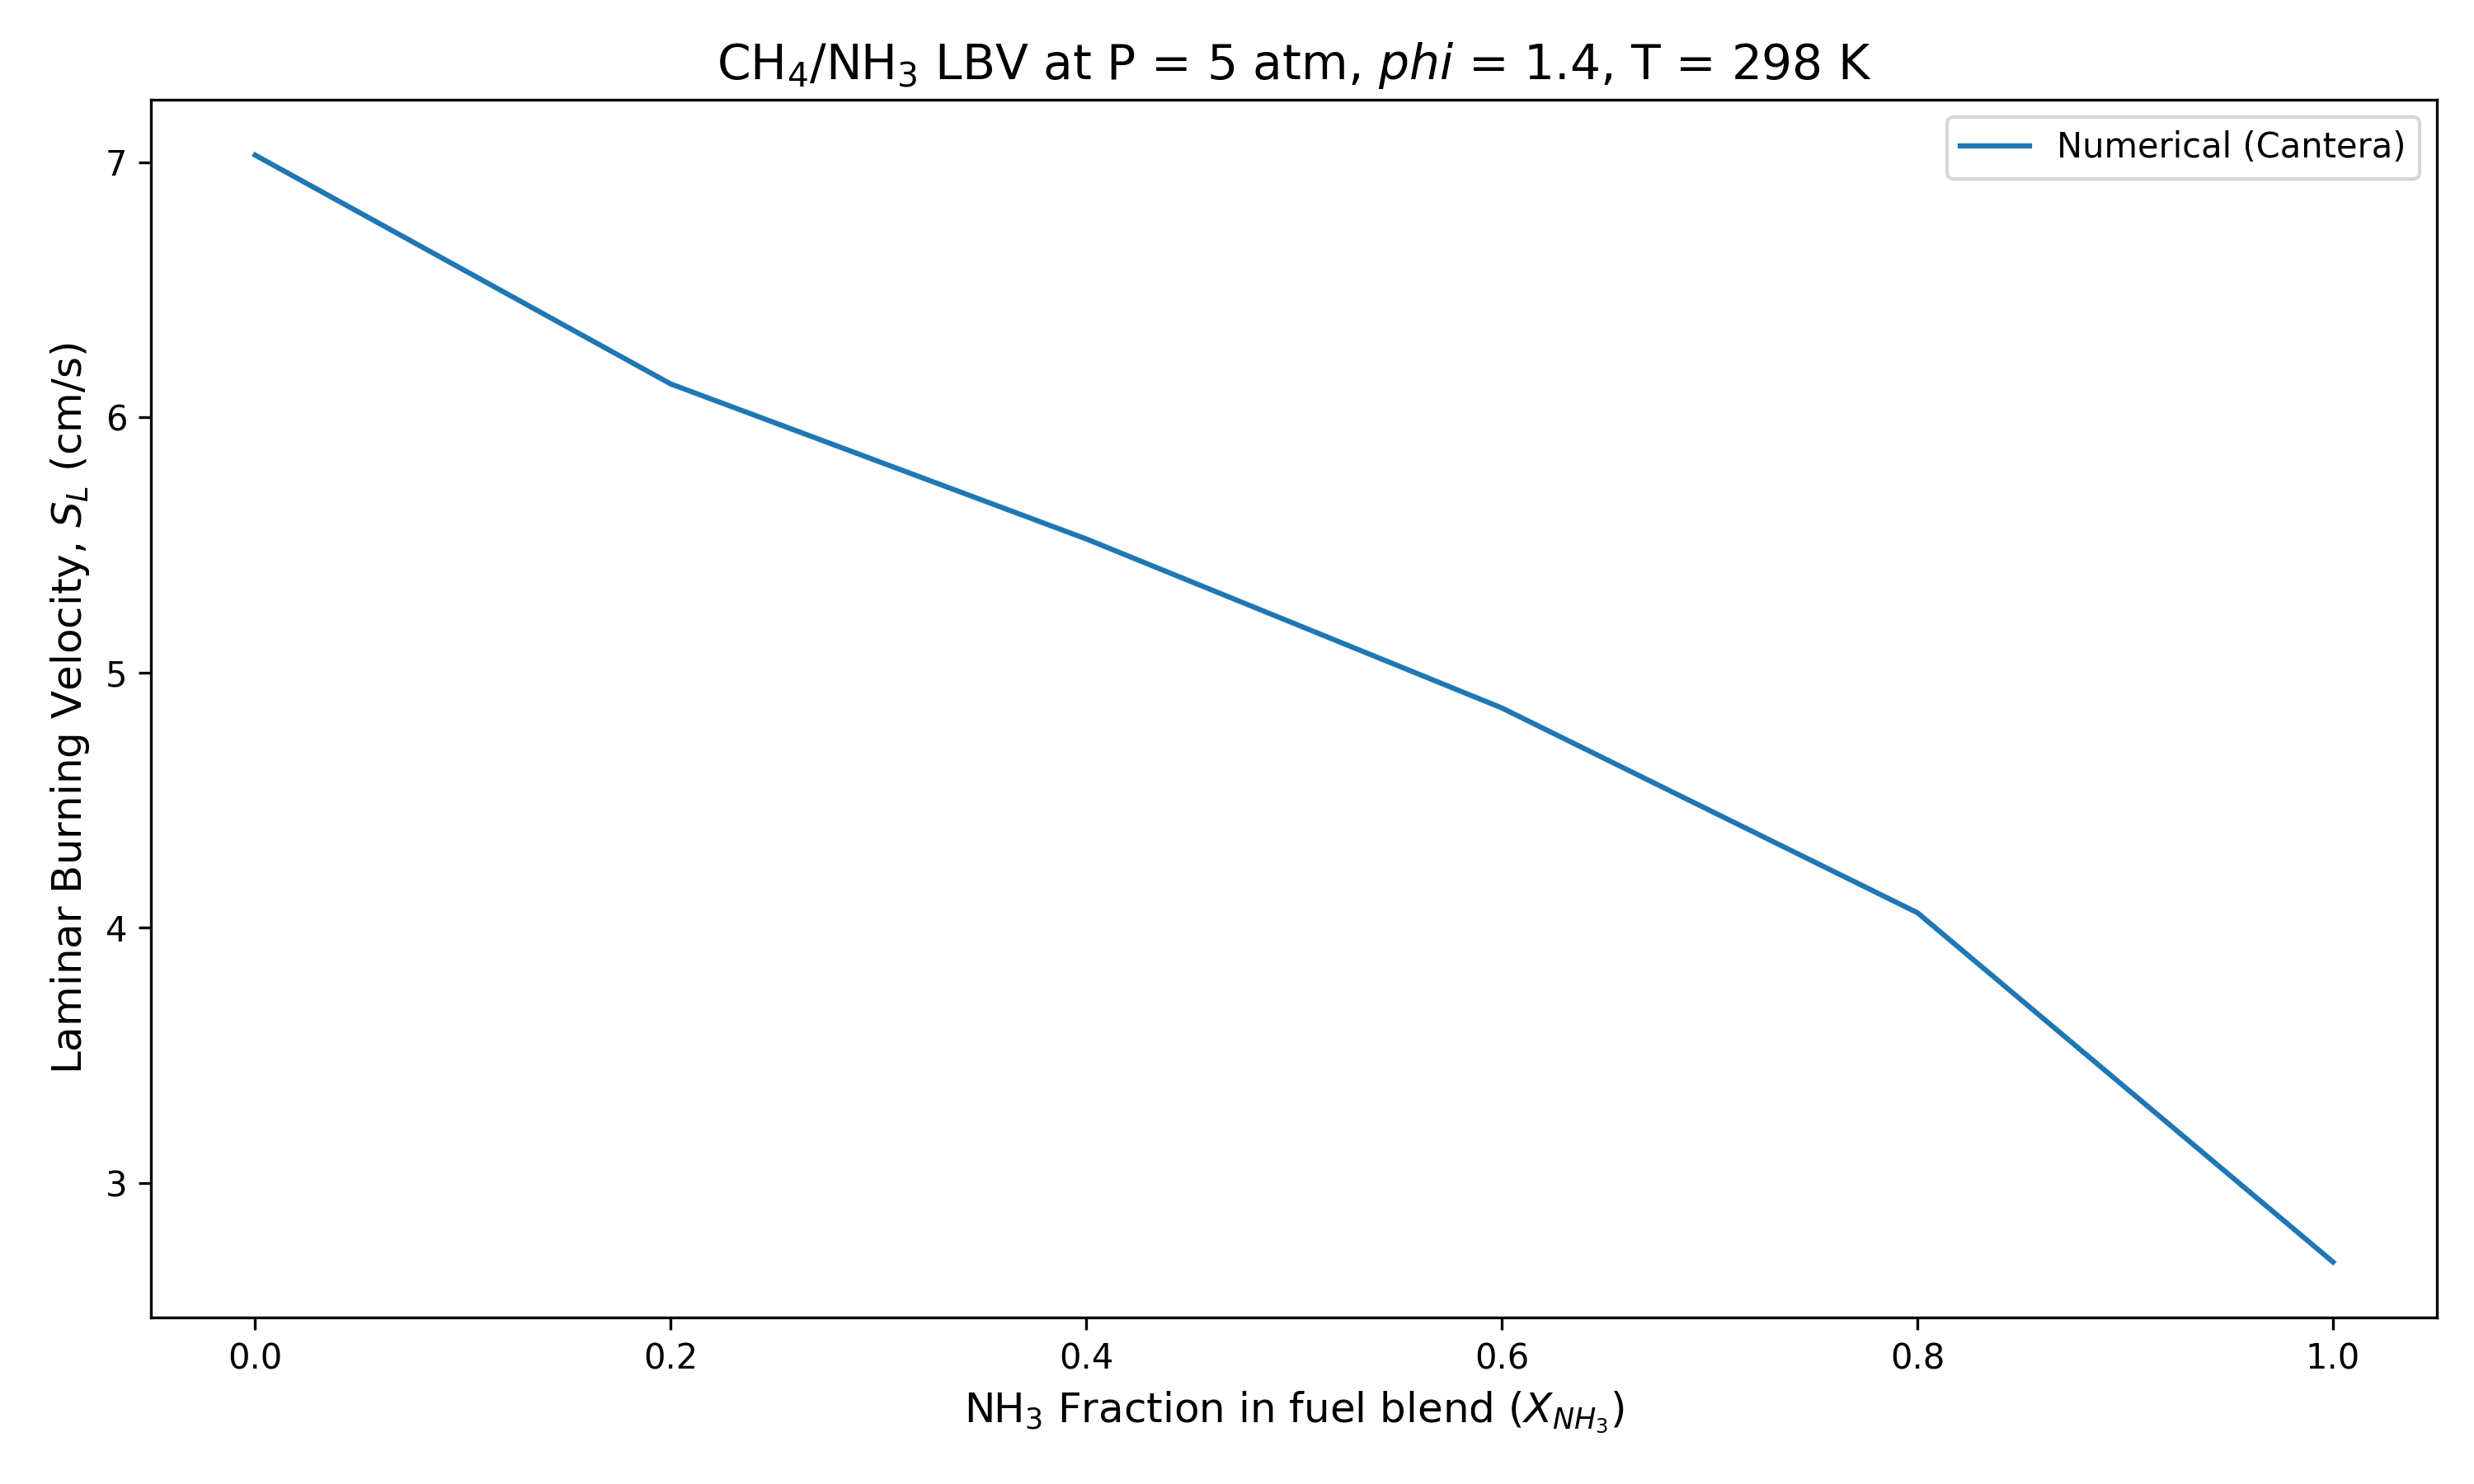
\includegraphics[width=\textwidth]{figures_ch4-nh3/lbv_p-5_phi-14.png}
			\caption{rich equivalence ratio}
			\label{}
		\end{subfigure}
	\end{figure}
\end{frame}

\begin{frame}{Remaining Objectives}
	\begin{itemize}
		\item Numerically evaluate species profiles with Plug Flow Reactor
		\begin{itemize}
			\item NO
			\item NH$_3$
			\item CO$_2$
		\end{itemize}
		\vspace{10pt}
		\item Numerically evaluate intermediate species profiles with Stagnation Flame Model
		\begin{itemize}
			\item OH
			\item NNH
			\item NH
		\end{itemize}
		\vspace{10pt}
		\item Optimize reaction mechanism to fit experimental data for all conditions above satisfactorily
	\end{itemize}
\end{frame}

\begin{frame}{References for Experimental Data}
	\tiny
	\fullcite{gotamaMeasurementLaminarBurning2022}
	\fullcite{shresthaExperimentalModelingStudy2021}
	\fullcite{wangExperimentalKineticStudy2021}
	\fullcite{wangExperimentalStudyKinetic2020}
	\fullcite{zhouExperimentalKineticModeling2023}
	\fullcite{hanExperimentalKineticModeling2019a}
	\fullcite{okafor2019}
	\fullcite{lingExperimentalKineticModeling2026}
\end{frame}

\end{document}
